\chapter{Щекавица и Лукьяновка}

Щекавице повезло. Её несколько раз упомянули в древней летописи – то относительно живущего на ней Щека, то как о месте захоронения Вещего Олега. И само название Щекавицы, искажаясь в Скавику, Скавицу, Шкавику, Щкавицу, дошло до наших дней да вернулось к Щекавице – и никому в голову не придет перенести ея на другую гору.

Щекавица лежит к северо-западу напротив Замковой, и на север от Воловни и Кудрявца. Между Щекавицей и Кудрявцем протекала речка Кудрявец, ныне известная как Глубочица. Начинаясь холмом к западу от Житнего рынка, Щекавица расползается в сторону Кирилловских высот на северо-запад к «новой» Юрковице (прежней Лысой), и на запад в сторону Лукьяновки, причем там уже трудно определить, где Щекавица заканчивается.

В 21 веке гора стала борзо застраиваться многоквартирными и частными домами-теремами. Беспощадно сносят старые домики. Склоны попросту срывают и «ук\-репляют». По горе проходят две основные улицы – Олеговская (с 18 века до 1869 года Погребальная) и Лукьяновская, названная так потому, что идет к Лукьяновке. А Олеговская по имени Вещего Олега, от его могилы, кургана.

В 19-20 века веках были на Щекавице и прочие улицы, например Черный яр. Жила память об урочищах: Волчий яр (на некоторых картах так обозначали удолье западнее старообрядческого кладбища, а жители называли Волчьим яром нынешнюю улицу Солевую), Чмилёв яр.

Сложно дать описание Щекавицы на 2014 год. Я часто стремлюсь ограничивать рассказ определенным временем, чтобы оставить память, да и не править главу каждый раз при изменении местности. Гора застыла в ожидании изменений, которые навсегда исказят её облик. Это уже случилось на отрогах вдоль оврага Глубочицы, где от стройки вечной склоны калечные.

Но есть и уснувшие уголки. Среди зеленого пустыря – битый кирпич стыка 19-20 веков, остатки фундаментов. Разрезанный пополам отрог на Лукьяновской улице, в нем – следы древней печи. Заброшенная строительная площадка\footnote{На 2016 год всё уже было построено, а от бывшего склона с печью остался жалкий кусочек. И никакой печи.}. Странные огражденные участки. Бывшая вышка-глушилка, ныне передающая FM-станции, нависает над всем. Выше неба!

\begin{center}
\includegraphics[width=0.88\linewidth]{chast-colebanie-osnov/sheka/\myimgprefix 27082009620.jpg}

\textit{2013. Домик в начале Олеговской улицы.}
\end{center}

От улицы Нижний Вал на холм лезет Олеговская улица, между новостроек и уцелевших старинных домиков, украшенных деревянной резьбой. Справа на пригорке, на прямоугольном охраняемом пространстве – вышка, посторонним ход заказан. За вышкой прячется северный отрог со следами древних укреплений. Улица поворачивает то направо, то влево. Название навевает вопрос – где же именно была Олегова могила?

Покамест вспомним утверждение Повести временных лет о Вещем Олеге: «и погребоша и на горе, иже глаголеться Щековица; есть же могила его до сего дни, словёт могила Олгова». «Погребоша и» – погребли его.

Невесть с чего наши современники иногда пишут, что змея укусила Олега здесь же, на горе. Но летописный Олег поехал «в поле», чтобы поглядеть на кости коня своего. Потом его укусила змея, он болел, затем его похоронили на Щекавице. В списках, гору называют также «Сщековища», «Щоковика». А в 19 веке в народе говорили просто «Скавика».

\begin{center}
\includegraphics[width=\linewidth]{chast-colebanie-osnov/sheka/\myimgprefix 27082009618.jpg}

\textit{2013. Старая застройка на Олеговской.}
\end{center}

Название «Олгова» встречается в летописи порой отдельно от Щекавицы. Вот Ипатьевский список, распря между Изяславом Мстиславичем и Гюрги (Юрием Долгоруким) за Киев в 1151 году:

\begin{quotation}
Вячьслав же, Изяслав и Ростислав повелеша Володимиру поити с Берендеи, и с вежами и с стады их пойти ко Олгове, и сташа мьжи дебрьми от Олговы оли (даже) и в огород святаго Иоана, а семо (сюда, здесь) оли до Щковице.
\end{quotation}

Вячьслав, Изяслав и Ростислав повелели Владимиру пойти с Берендеями к Олгове. И Владимир с Берендеями стали между дебрями от Олговы да в ограде церкви святого Иоана, и до Щковицы.

Тут ясно разделяются местности – Олгова и Щекавица. В летописях князья часто ездят к именно Олговой могиле, а Щекавица вот упомянута, кроме захоронения Олега и места жительства Щека, только в приведенном куске про Берендеев.

Если моё толкование верно, речь идет о двух смежных местностях, Щекавице и Олгове могиле. Возможно, одна часть горы называлась Щекавицей, а другая – Олгова могила. Хотя Нестор пишет, что Олгова могила находится на Щекавице. Лашкарев в 19 веке, по его словам, слышал, как Ольговой могилой именовали мыс над Вознесенским спуском на Кудрявце, то есть напротив современной Щекавицы.

О церкви святого Иоанна, за год 1121 летопись сообщает: «Того же лета заложи церкви святаго Ивана в Копырев Конци». Закревский, принимая эту церковь за ту же, про кою говорилось касательно Берендеев, делает вывод – местность Копырев Конец тоже находилась на Щекавице. Замечу, летопись упоминает сию церковь с привязкой к двум местам – Олгове и Копыреву концу, не к Щекавице. Про Копырев конец подробно отсылаю вас в часть этой книги про Логово змиев, глава «Копырев конец». Мы же пока не сходим с Щекавицы.

Киевский епископ (1592-1598 годы) Иосиф Верещинский (аббат Сецеховский) в конце 16 века, желая затеять стройку века и заодно расширить владения доминиканов, написал к депутатам сейма обращение «Способ заселения Нового Киева и обороны бывшей столицы киевского княжества от всякой опасности без обременения его величества короля и без затрат для короны польской, объясненный господам послам будущего краковского сейма»\footnote{Sposob Osady Nowego Kijowa y ochrony niegdy Stolice Księstwa Kijowskiego od niebespieczeństwa wszelkiego [...] Panom Posłom na Seymie Krakowskim przyszłym podany Przez [...] Iozepha Wereszczynskiego [...].}, напечатанное книжечкой в 1595 году. Его перевод помещен в мартовском нумере «Киевской старины» за 1894 год.

Там мы находим важнейшие сведения, ибо Верещинский был очевидцем двух, как сказано в переводе «кремлей» (крепостей в городской черте) – одного на Щекавице, другого на некой противоположной горе, и что на Щекавице обитали иудеи. Значит, летописное урочище «Жидове»\footnote{Так раньше называли иудеев.} и есть Щекавица?

Епископ в описаниях, которые мы разберем далее, при сравнении упоминает названия краковских урочищ, а из киевских называет лишь одно – Щекавицу. Другая важная в его и моем повествовании гора у Верещинского остается безымянной, про нее он говорит не иначе как про место кремля Кия. Замковая гора тоже остается без названия, просто как гора, где стоит современный епископу замок из гнилого дерева.

Поэтому мы можем, думаю, доверять сведениям Верещинского в описательной части, но как быть с исторической связью, допустим, Кия с упомянутым кремлем? Насколько верно соотносит епископ гору, на которой расположена давняя земляная крепость, с Кием? Мы знаем множество примеров ошибочных сопоставлений, ну вот как считал Рыбаков Андреевский спуск увозом Боричевым.

Но довольно, буду рассуждать по ходу. 

Вначале епископ отрицает истинность расхожего тогда мнения, что Киев прежде был Троей, затем рисует картины запустения Верхнего города, где среди развалин Софии пасутся свиньи, и далее сообщает:

\begin{quotation}
К тому же Киев (Kyow) имел собственных земель пространством более, чем на 50 польских миль, и два стольных кремля, расположенных друг против друга и принадлежавших двум родным братьям, Кию (Kiy) и Щеку (Sczyk). Они и теперь еще стоят пустыми, окруженными огромными земляными валами.

Валы эти, если бы нанимать грабарей, с большой натяжкой едва ли можно было бы насыпать за 500,000 червонцев.\footnote{1,5 миллиона рублей в 1894 году, что означает небывалый масштаб остатков древней фортификации, которую застал Верещинский.}

Один из этих двух пустых кремлей захватывает такое пространство, какое – краковские стены со всем своим замком. Этот киевский старинный кремль, запущенный еще до тех пор, как началось процветание киевской столицы, имеет валы такой высоты, как костел св. Станислава в краковском замке.

Что касается другого кремля, который и теперь еще стоит, то всегда после его разрушения еще во времена язычества, и после смерти бездетного упомянутого выше Щека, родного брата Кия, он был заселен жидами.
\end{quotation}

Итак, Верещинский пишет о сохранившихся крепостях, стоявших друг против друга в запущенном состоянии. На Щекавице, как понимаю, состояние лучшее, ибо «и теперь еще стоит», и эта крепость Щека была разрушена еще до крещения Руси. 

А вот запустение «киевского старинного кремля» – коим, по словам епископа, владел Кий – почему-то началось с процветанием «Киевской столицы». 

Первый кремль, Кия, епископ сопоставляет по площади с «краковскими стенами со всем своим замком». В современном состоянии замок Вавель в Кракове по карте можно определить условно как 320x160 метров. Такого размера крепость не могла стоять на относительно мелкой горе вроде Клинца или Уздыхальницы. По некой причине место «кремля Кия» больше не заселяли, вернее, при епископе он пребывал в запустении.

А вот Щекавица другое дело. Бездетный Щек умер, и его крепость заселили иудеи. Однако,

\begin{quotation}
С введением христианства, по убеждению апостола Киевского св. Яцка\footnote{Доминиканский монах Яцек (Иакинф) Одроваж, по прозвищу Гиацинт (Sancti Iacchonis, 1183-1257), проповедник католицизма в Киеве в 1222-1226 годах. «По убеждению апостола» значит, что его стараниями.} они были изгнаны оттуда, так как замучили для своих жидовских суеверий христианское дитя, а их местожительство вместе с упомянутым кремлем отдано было польскими королями кафедре киевского бискупства\footnote{Как видим, старания святого Яцека принесли ощутимую выгоду доминиканам. Слово же «кафедра», вероятно, искаженный перевод «катедры», то бишь католического кафедрального храма, кафедрального костёла.}.

Этот кремль и теперь называется жидовским городом;\footnote{То бишь после изгнания оттуда иудеев, еще три века в народе держалась молва о прежних обитателях Щекавицы!} он разделен в середине на две половины двумя огромными валами, а вокруг обсыпан также огромным валом вышиною, как костел св. Станислава в краковском замке; ширина и длина его, как Страдом между Краковом и Казимиром.
\end{quotation}

Страдом в то время – урочище в Кракове южнее Вавельского замка, упрощенно 700x220 метров. Это вполне соотносится с Щекавицей считая от восточной ее стороны и эдак по Старообрядческое кладбище.

Бискуп относит виденные им масштабные укрепления ко временам Кия и Щека. Получается, летописные братья имели возможность развернуть на холмах строительство, выходящее за обычное представление науки о небольшой деревянной крепости.

Итак, где-то на Щекавице была крепость Щека, разделенная посередине двумя огромными валами, и вокруг крепости еще один вал высотой с костел святого Станислава. Сейчас почти вся Щекавица застроена, да и прежде застраивалась, перекраивалась – мы не знаем, какие валы были срыты, например, при устроении Щекавицкого кладбища.

Очевидно, что этот «кремль» находился на плато Щекавицы, но где? Остатки неких валов существуют на северо-восточном углу Щекавицы, а почти прямоугольные очертания той части горы (как и противоположной Замковой) свидетельствуют о колоссальных земляных работах в глубоком прошлом. Именно таких валов, как описал Верещинский, я не находил. Проскальзывает еще мысль, что некоторыми высоченными валами Верещинский считал сами рукотворно ровные склоны.

Епископ предлагает:

\begin{quotation}
Необходимо подумать, чтобы эти два огромных опустелых старинных кремля могли заселиться людьми без всяких расходов для Его Величества Короля и без обременения для республики; чтобы эти люди охраняли огромные валы от пограничных неприятелей и защищали почтенную столицу от различных опасностей, а особенно от князя московского.
\end{quotation}

Далее Верещинский рассказывает о киевском замке на Замковой горе, различая его и гору с «кремлем» Кия (отметка жирным шрифтом – моя):

\begin{quotation}
К тому же следует укрепить и теперешний замок, который расположен на довольно высоком холме; холм под теперешним замком, наполовину изгнившим, имеет сам по себе высоту краковской ратуши, а по ширине и длине он соответствует краковскому замку со всем его пригородом.

Вот этот-то теперешний замок на вышеупомянутом холме, по природе высоком, должен быть возобновлен, \textbf{но своим порядком должно быть устроено поселение на месте пре\-жнего княжеского двора, на том роскошном холме, где князь киевский, названный Кием, имел свои великолепные палаты}.
\end{quotation}

Надо починить существующий замок на Замковой горе (Киселевке), а отдельно устроить поселение в крепости, где был княжий двор Кия.

\begin{quotation}
Другая гора от природы высока, похожа на упомянутую Киеву гору и не уступает ей по ширине и длине. 
\end{quotation}

Другая гора – имеется в виду Щекавица.

\begin{quotation}
Эти две горы, как брат с сестрой, стоят на расстоянии друг от друга, какое занимает краковский рынок. Вторая гора называется бискупской горой или Щекавицей, от князя Щека, родного брата князя Кия.

На этой горе он имел свой особый двор, очень роскошный, от которого теперь нет и признаков. Гора эта должна быть обращена в бискупский замок для его кафедры, так как она не может быть застроена никак именно, кроме самого Его Величества Короля или киевского бискупа\footnote{О Верещинский, о лукавый бискуп!}. Эти две горы, равные высотой, если будут укреплены стеной и строениями, то будут служить одна другой опорой в годину опасности от неприятеля Короны Польской.
\end{quotation}

Теперь остановимся и рассудим. Можно ли по описанию епископа вычислить, какую гору он полагает местом кремля Кия? Вне зависимости от того, в самом ли деле это была гора Кия. Обозначим ее горой Икс.

Сказано, что гора Икс находится напротив Щекавицы, эти две горы как брат с сестрой, и расстояние между ними подобно краковскому рынок. Сейчас площадь Rynek Główny в Кракове имеет квадратную форму с шириной стороны около 160 метров.

Прикинем.

Можно сказать, что по разные стороны непосредственно напротив Щекавицы лежат четыре горы (Воловня не катит). Это исконная Юрковица (отрог со Старообрядческим кладбищем). Новая Юрковица (прежде Лысая). Замковая. Кудрявец. На одной из них, по словам бискупа, был кремль Кия. Замковую исключаем, поскольку Верещинский говорит о ней, как про отдельную гору, не ту, где расположен кремль Кия, а ту, где стоит существующий гнилой замок.

Значит, выбор сводится к трем вариантам – Кудрявец, исконная Юрковица и Юрковица-Лысая. Первый в протяженности напротив Щекавицы не больно уж крут и неприступен, чтобы служить естественной крепостью. Да и не приходит в голову сравнить Кудрявец и Щекавицу с братом да сестрой.

Поскольку на Юрковице-исконной (отрог с кладбищем старообрядцев) обитал Хорив, о чем вы прочтете в части про Кирилловские высоты, остается одно – горой с кремлем Кия епископ полагал гору Лысую, ныне именуемую Юрковицей.

Как это согласуется с моим предположением, что хотя Кий отдельно обитал на горе «идеже ныне увоз Боричев», но общая с братьями крепость Киев была построена на Лысой, я разбирать не буду. Пробовал, но это завело меня в краеведческий тупик. Я не могу перенестись в 1695 год, ходить с епископом по холмам и спрашивать его – как эта гора называется? А откуда вы узнали, что эти фортификации относятся именно к Кию? Кий был тут до устроения общей крепости или наоборот, тут находилась уже общая крепость братьев?

В своем проекте Верещинский предлагал, чтобы Киев состоял из трех частей-городов. Первая это Подол и гора Замковая с полусгнившим старым деревянным замком, который нужно привести в порядок. Другой город, крепость – высотный, на бискупской горе, которую он соотносит с Щекавицей. Там дескать бывший кремль Щека и огромные валы, надо только башни поставить. Наконец третий город – на другой горе, на месте бывшего «кремля Кия». Тут Верещинский прочит устроение замка короля. Привычный же нам «верхний город» с Софией и прочим при Верещинском пребывает в развалинах и запустении, он не в счет.

Словесная картина Верещинского, ясная ему самому, для меня путаная, путаницу вносит гнилой замок, «нынешний стольный замок Его Величества». Он в описываемые годы есть, на Замковой горе, установленный факт. И где-то рядом стоят еще две горы, на доной кремль Щека (Щекавица), на другой кремль Кия.

И вот еще зацепка от Верещинского, и она сводит меня с ума:

\begin{quotation}
Этим способом, милостивые государи, каждый поставлен был бы в изумление, что отважился бы наступать на главный киевский замок Его Королевского Величества, который был бы зеницей в глазу, занимая средину между стародавним Киево-Подолом и двумя новыми городами, поселенными в упомянутых огромных валах, ему могло бы быть оказано необходимое подкрепление в случае надобности со всех трех сторон.
\end{quotation}

Гнилой замок на Замковой горе, стало быть сама Замковая гора, находится посередине между Подолом и «двумя новыми городами». При этом Щекавица должна быть «как брат с сестрой» с какой-то другой горой, горой Кия, однако я не вижу никакой горы смежной одновременно с Щекавицей и Замковой, причем такой горой, которая будет «как брат с сестрой» с Щекавицей!

Во время, когда бискуп Верещинский желал расширения владений, и когда Киев был под Литвой да Польшей, Щекавица впервые после летописей появляется в источниках, а именно в земельных документах – как местность, где расположены пахотные нивы и пастбища. На южной стороне горы, напротив Киселёвки, в 16 веке зеленел виноградник.

В 1619 году Сигизмунд III жалует Щекавицу, по их челобитью, киевским мещанам на «осаживание людей», дабы гора населялась и город расширялся. Границы передаваемого «грунтика» определяются так:

\begin{quotation}
гору Щекавицу, з ея принадлежностями, почавши от Юркового ставка, потом в гору Щекавицу, от Оболонья отираючися о грунт, о дом и острог бискупий, в конец гребли; а от конца гребли в ставок в долину Кудрявец, до самого конца Кудравца, а от конца Кудравца просто чрез дуброву до борку Святошицкого, по дорогу, которая идет з Белгородки до Киева, а дорогою идучи до Киева, пришовши к концу долины Юркова ставка, в долине Юрков ставок, откуда началась граница
\end{quotation}

Юрков ставок с большой вероятностью отождествляется с удольем Нижнеюрковской улицы близ ее подъема на гору, «долина Кудрявец» с улицей Глубочицкой, а «борок Святошицкий» с окрестностями Святошина.

В 1770 году в Киев пришла чума. На верху Щекавицы начали спешно хоронить подольских умерших, равно как и просто во дворах, близ жилья.

Как раньше, при добрых царях, с чумой боролись? В основном – окружали район войсками и никого оттуда не выпускали. Так люди и умирали семьями. Кого-то вывозили в карантин на Труханов остров, и там здоровые соседствовали с больными. Обычно дома, куда заглянула чума, сжигались. Но Подол был столь тесно застроен, что сжечь там один дом значило бы распалить пожар повсюду. Когда чума перебралась в другие районы, включая верхний город и даже Зверинец, не пострадали одни лишь монахи Михайловского монастыря – они попросту заперлись за его стенами и никого не впускали. Между тем как в соседней Софии усопли 50 монахов и 70 певчих.

Спустя два года на Щекавице разрешили хоронить уже официально. Далее, в 1782-м, там появилась церковь Всех Святых (колокольню с острым шпилем к ней пристроили в 1809). Примерно на ее месте сейчас\footnote{50°27'58.9"N 30°30'21.1"E} – здание в 25 метрах на восток от вышки. В свое время церковь зарисовал приятель Тараса Шевченко, художник Михаил Макарович Сажин. Он написал множество пейзажей Киева 1840-50 годов. Снимал жилье в одном доме с Шевченко и Афанасьевым-Чужбинским на Козьем Болоте у нынешнего Майдана, в доме Ивана Ивановича Житницкого 1835 года постройки. Там сейчас музей Кобзаря.

\begin{center}
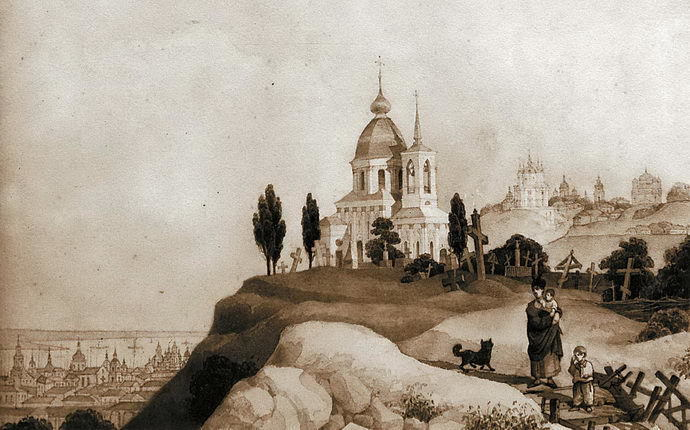
\includegraphics[width=\textwidth]{chast-colebanie-osnov/sheka/shekavica-sajin.jpg}

\textit{М. Сажин, Щекавица, 40-е годы 19 века.}
\end{center}

Эта картина Сажина – наиболее раннее известное мне изображение церкви на Щекавице. По некой причине художники, как увидим далее, предпочитали писать эту церковь в определенном ракурсе, глядя примерно на юго-восток, как бы зайдя с тыла. Видим покосившиеся кресты, небольшие деревца. Люди справа внизу, кажется, стоят около некоего мостика через провал в земле. 

Почти с того же месте изобразил церковь Всех Святых в начале 1850-х загадочный Генрих Гроте, оставивший после себя с полдесятка пейзажей Киева того времени, несколько лет проработавший художником рисования в Институте Благородных девиц, и вероятно служивший инженером при постройке Николаевского цепного моста.

Разница с картиной Сажина – с десяток лет. Помним, что мы глядим не на фотографии, а на художественные произведения, которые могут не точно изображать местность. На картине Гроте меньше намогильных крестов, деревца всё такие же чахлые, более понятна поверхность – суглинистый обрыв, невысокая трава (против нынешнего разнотравья).

\begin{center}
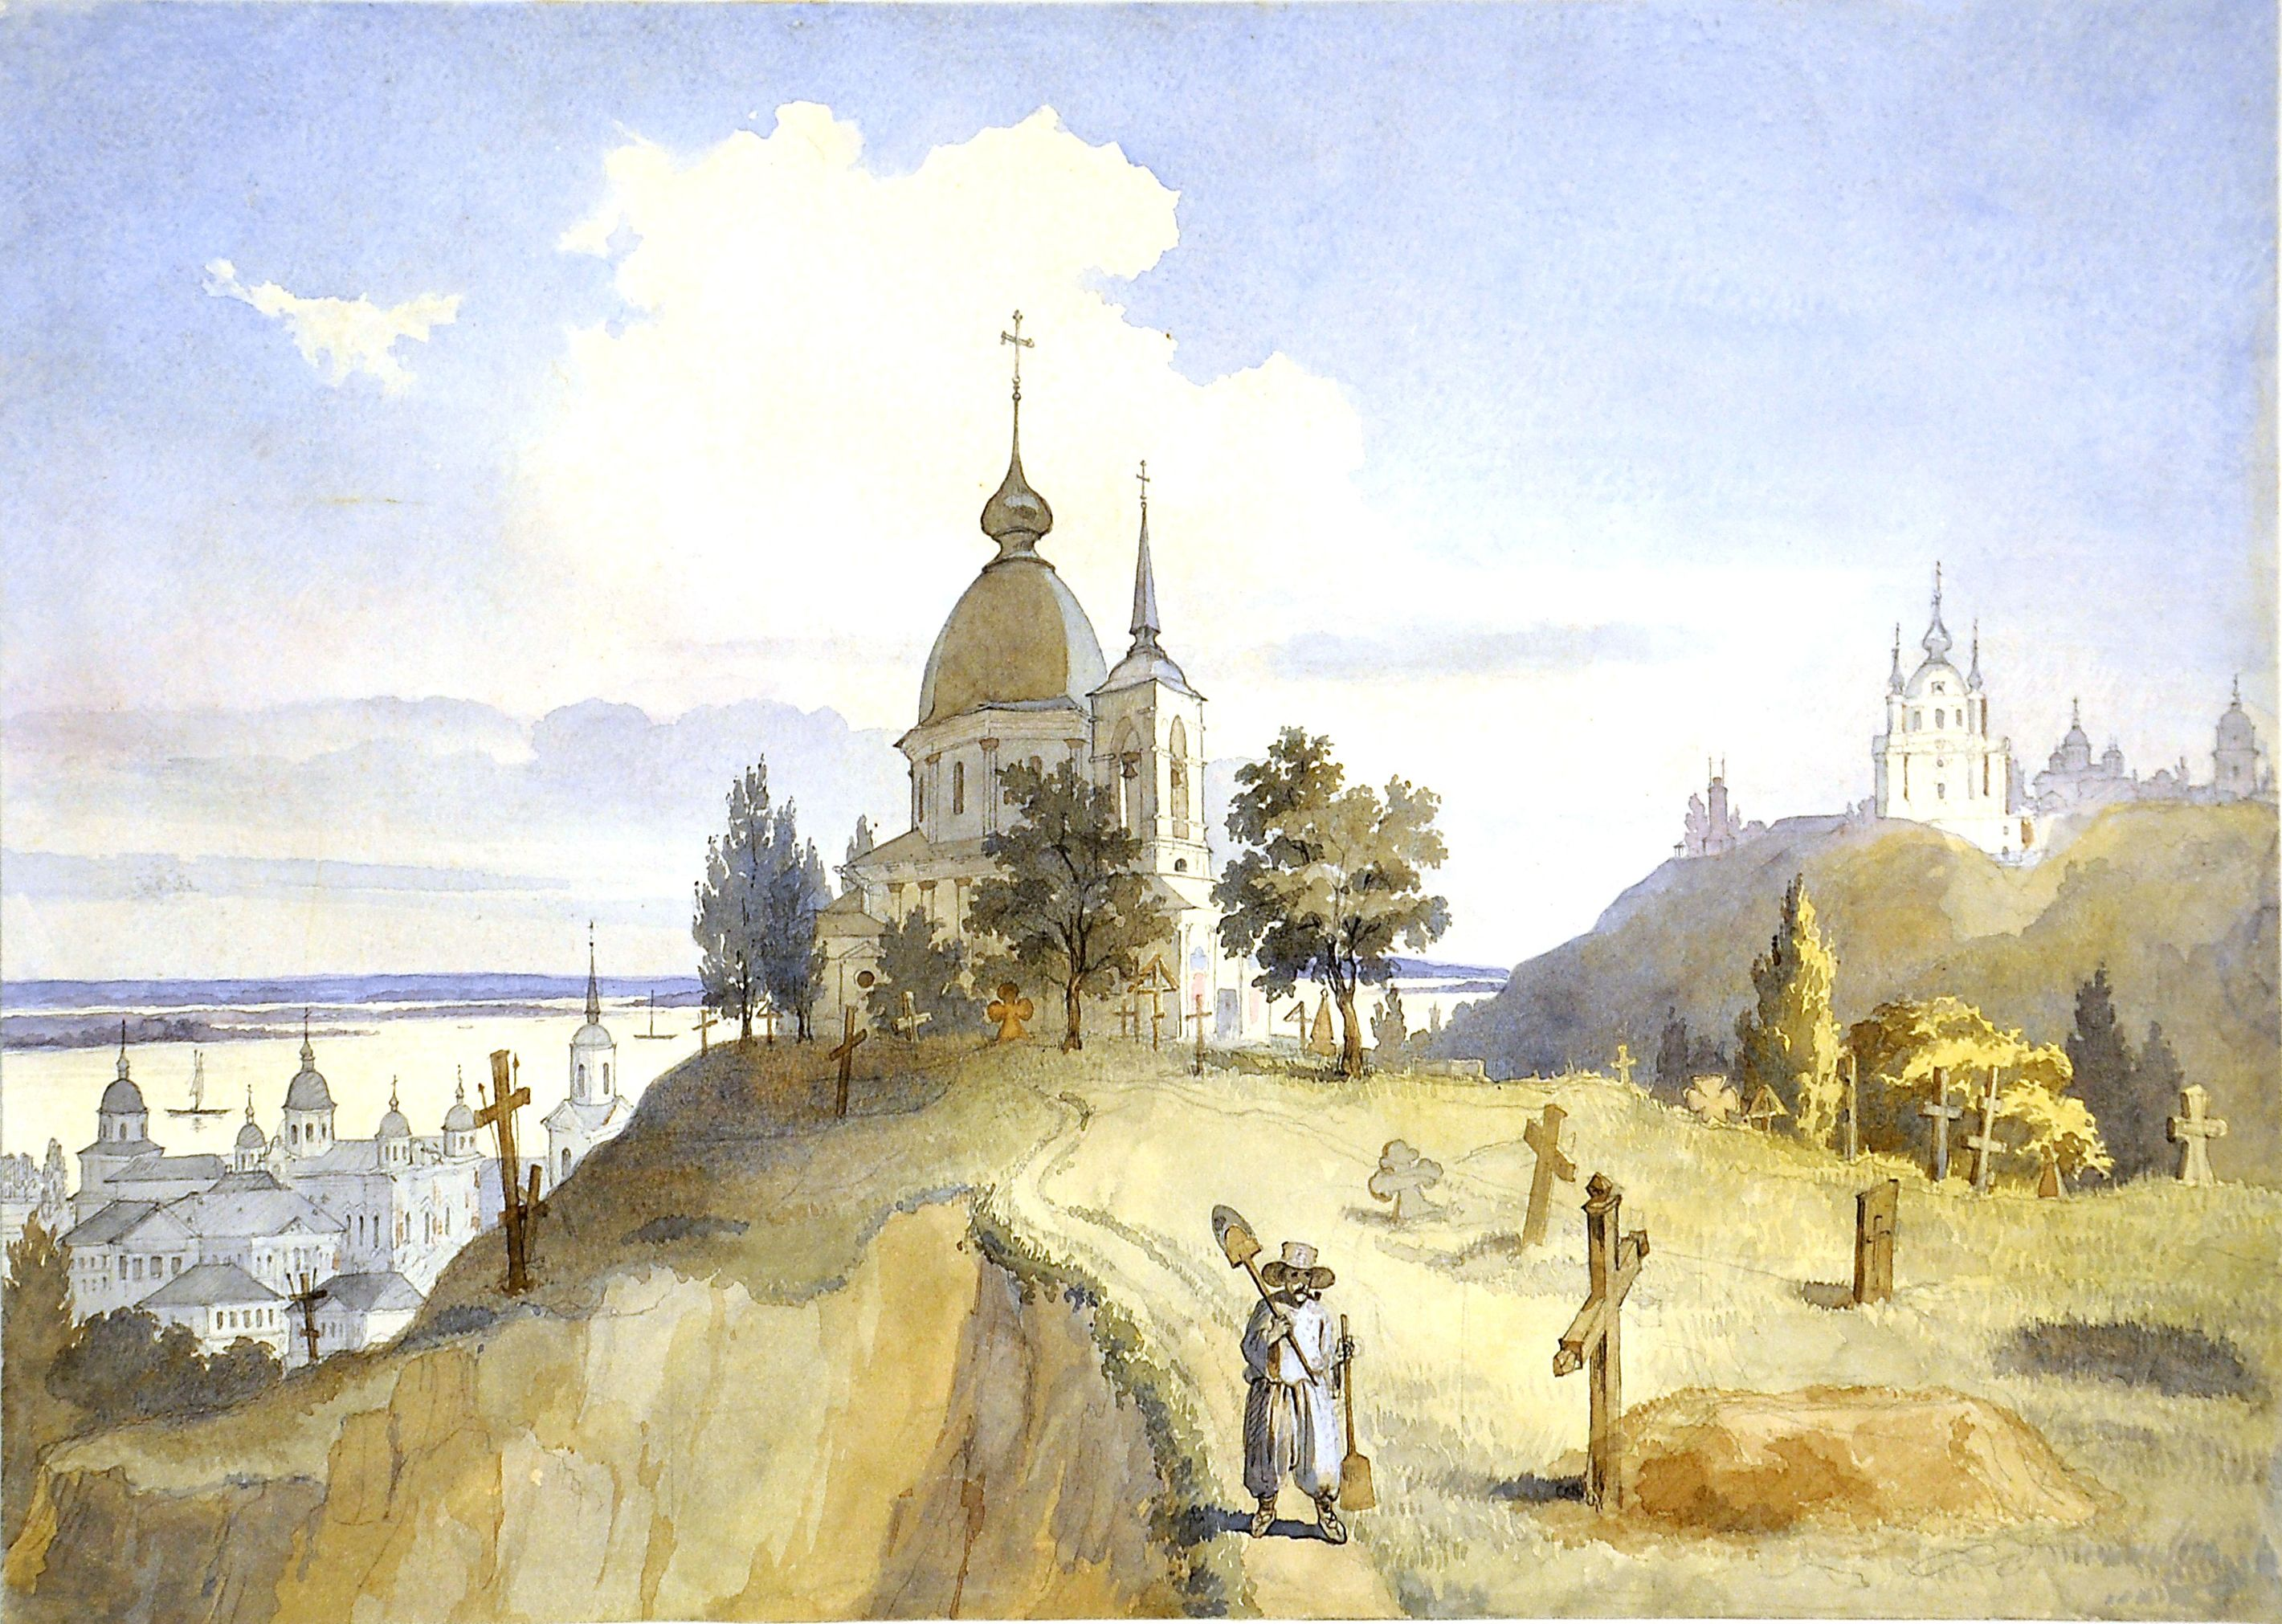
\includegraphics[width=\linewidth]{chast-colebanie-osnov/sheka/grote.jpg}

\textit{Генрих Гроте, начало 1850-х.}
\end{center}

%\begin{center}
%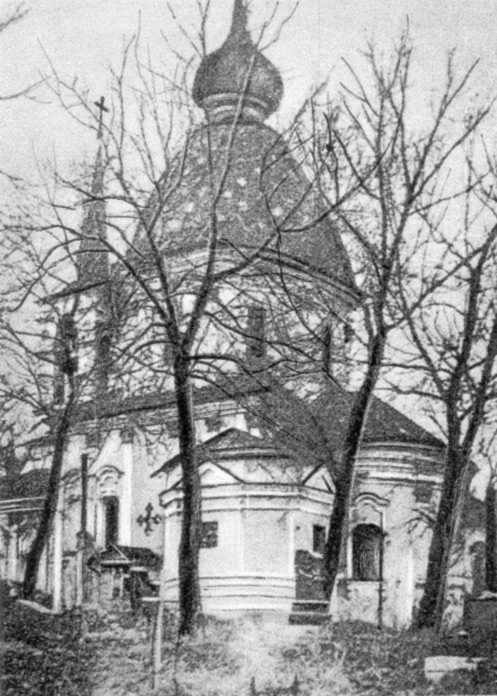
\includegraphics[width=0.50\linewidth]{chast-colebanie-osnov/sheka/vseh.jpg}

%\textit{Церковь Всех святых.}
%\end{center}



\begin{center}
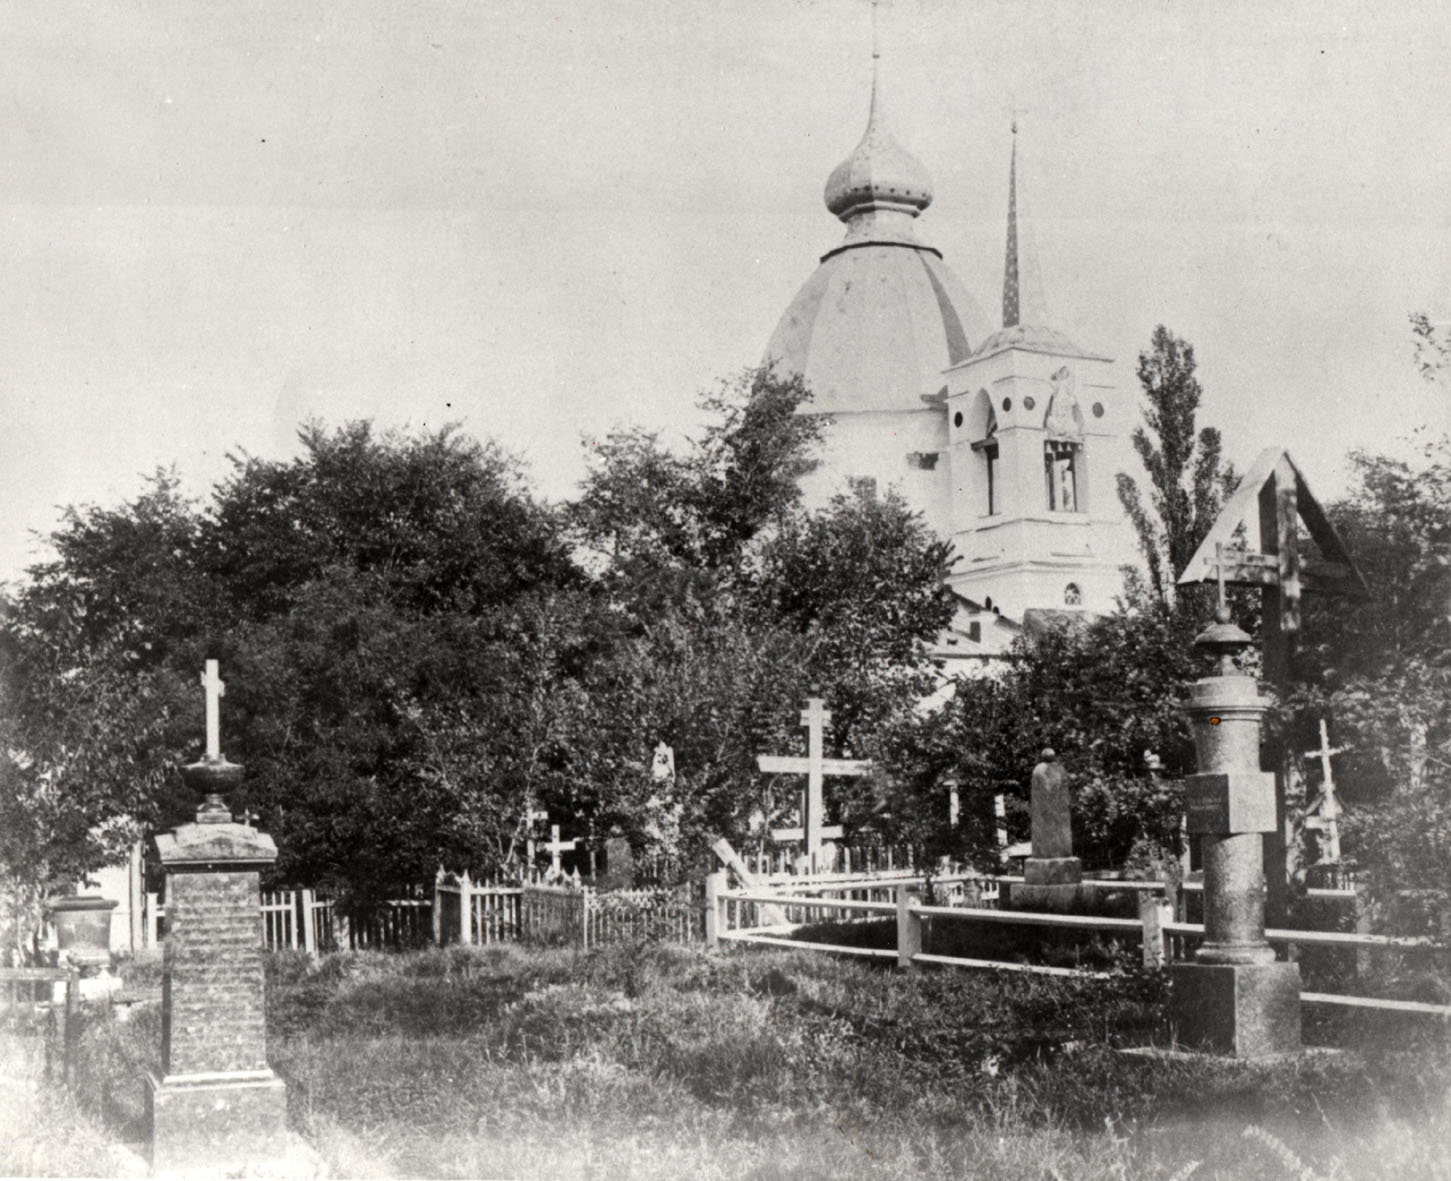
\includegraphics[width=0.70\linewidth]{chast-colebanie-osnov/sheka/sheka_kladb2.jpg}

\textit{Дореволюционный снимок кладбища на Щекавице.}
\end{center}


Далее снимки Щекавицы разных лет, сделанные с Киселёвки. Не совсем с одного места, но для сравнения подходят. Узнаваем изгиб Олеговской улицы, а улица Нижний вал в самом низу.

\begin{center}
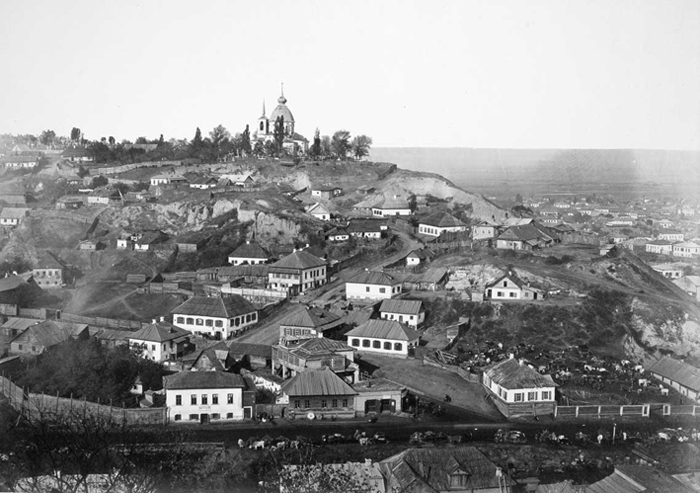
\includegraphics[width=0.90\textwidth]{chast-colebanie-osnov/sheka/sheka-19st-02.jpg}

\textit{Конец 19 столетия.}
\end{center}


\begin{center}
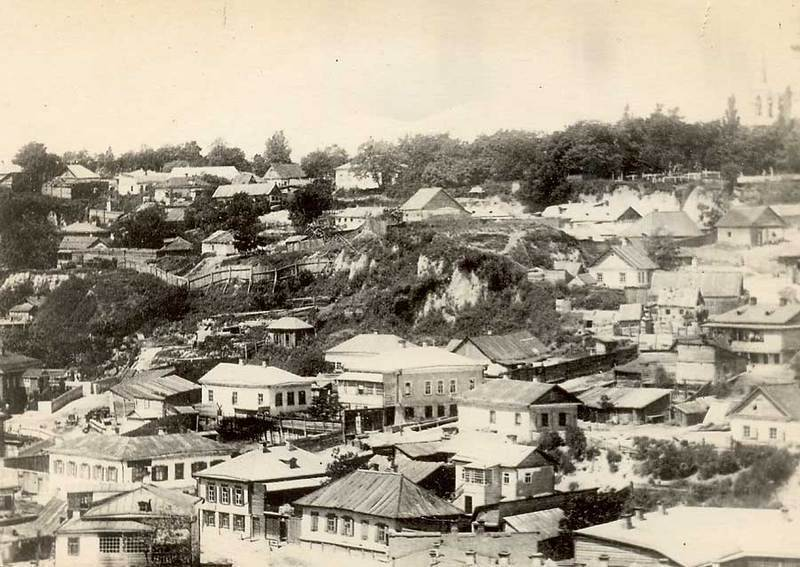
\includegraphics[width=0.90\linewidth]{chast-colebanie-osnov/sheka/sheka-19st-01.jpg}

\textit{Примерно то же время.}
\end{center}

\newpage


\begin{center}
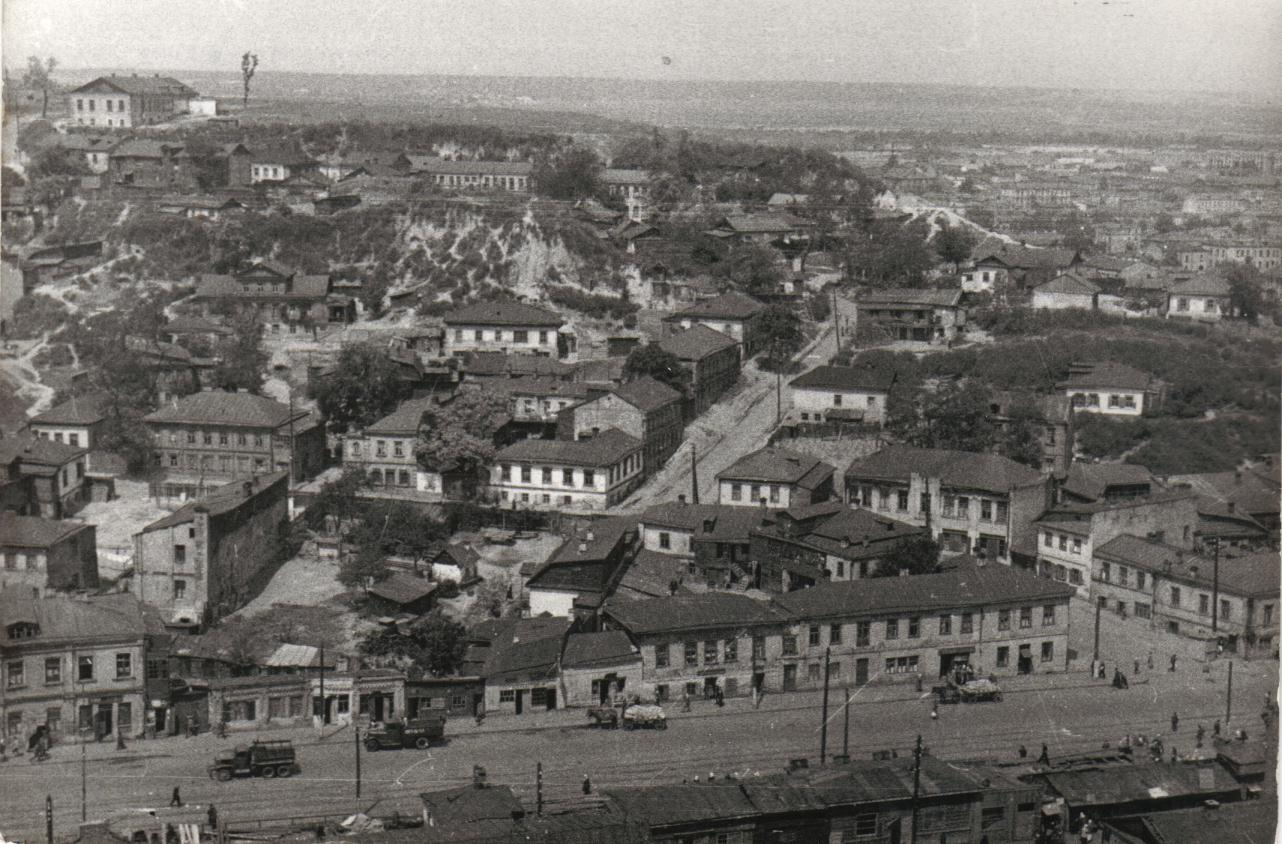
\includegraphics[width=0.98\textwidth]{chast-colebanie-osnov/sheka/sheka50.jpg}

1950-е.
\end{center}

\vspace*{\fill}
\begin{center}
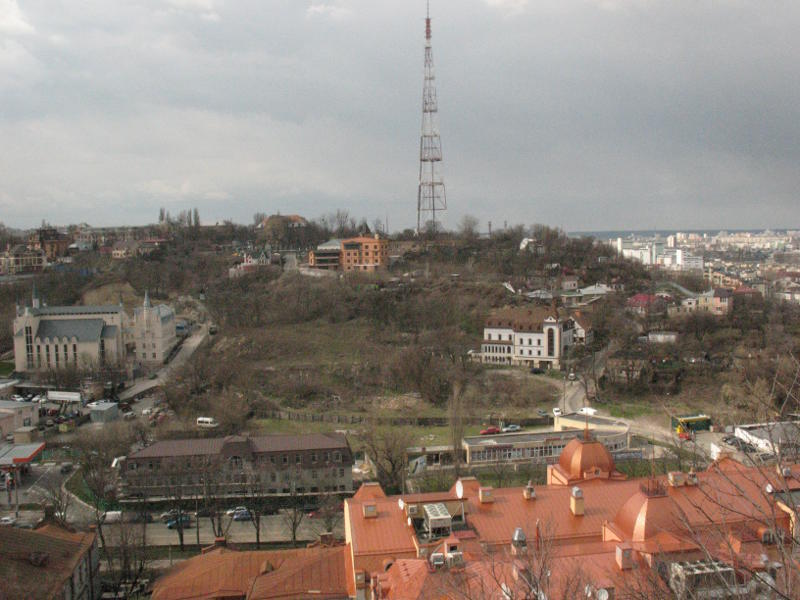
\includegraphics[width=0.95\textwidth]{chast-colebanie-osnov/sheka/sheka-now.jpg}

\textit{Апрель 2011.}
\end{center}

\vspace*{\fill}


%\begin{center}
%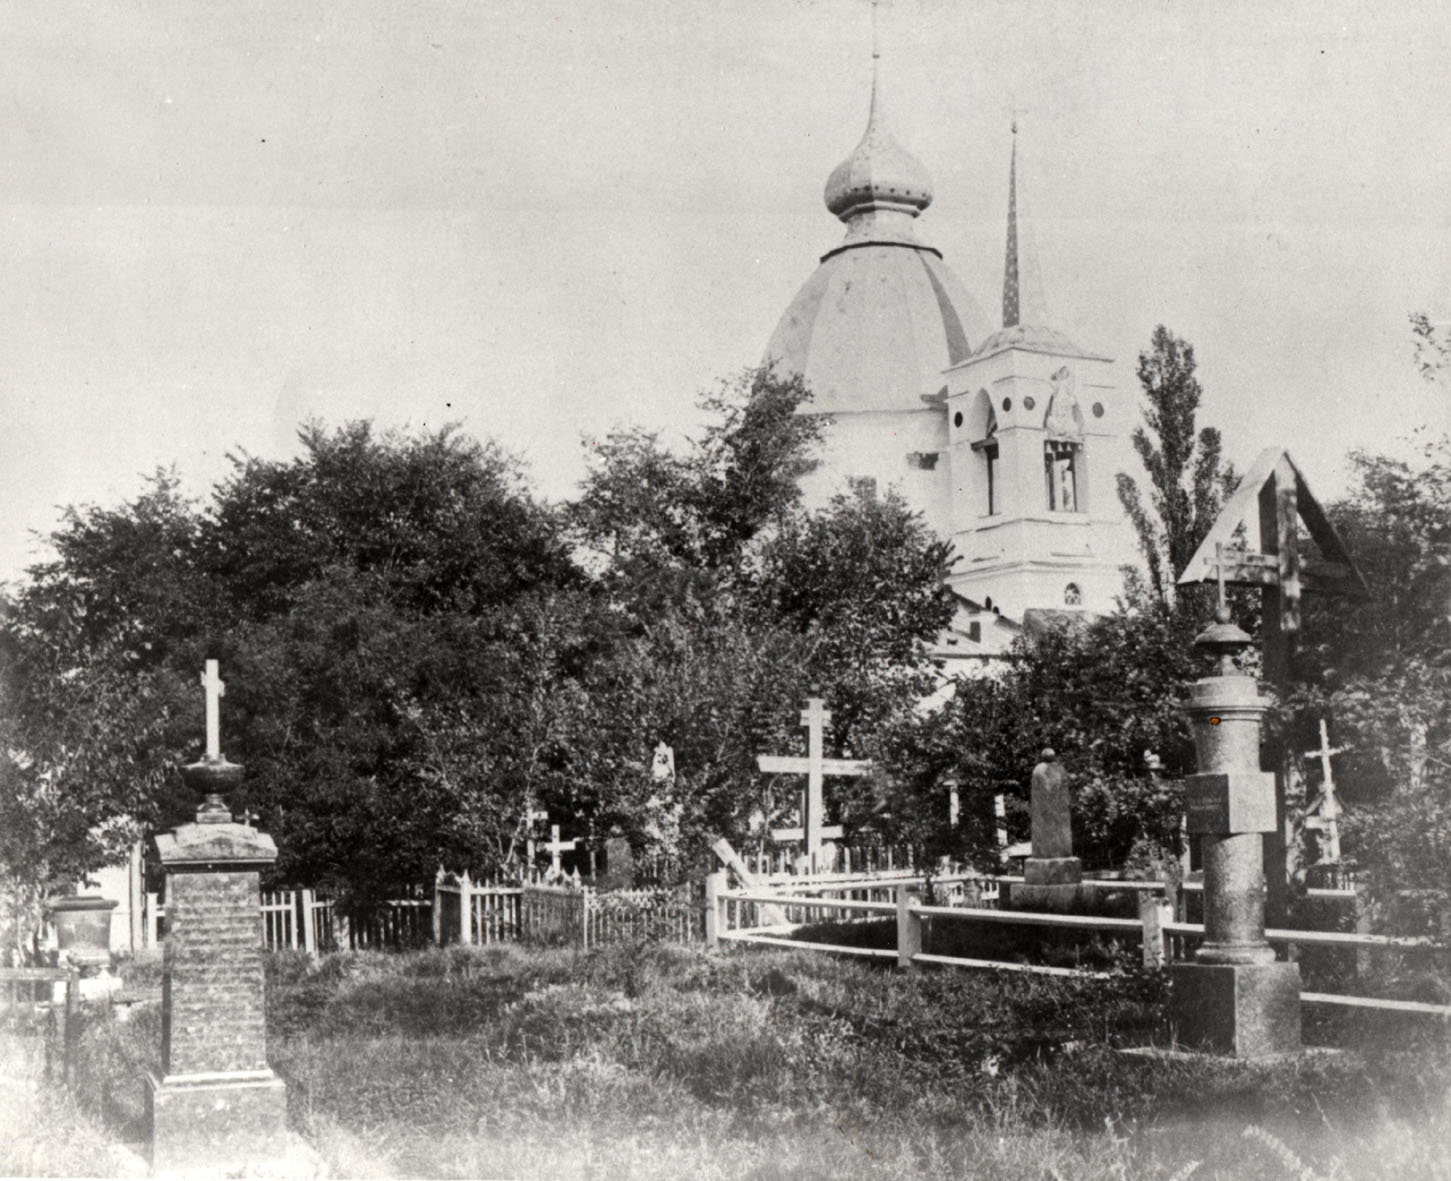
\includegraphics[width=\textwidth]{chast-colebanie-osnov/sheka/sheka3.jpg}

%\textit{19 век, ближе к Житнему торгу.}
%\end{center}
%\vspace*{\fill}

\newpage

%\vspace*{\fill}
%\begin{center}
%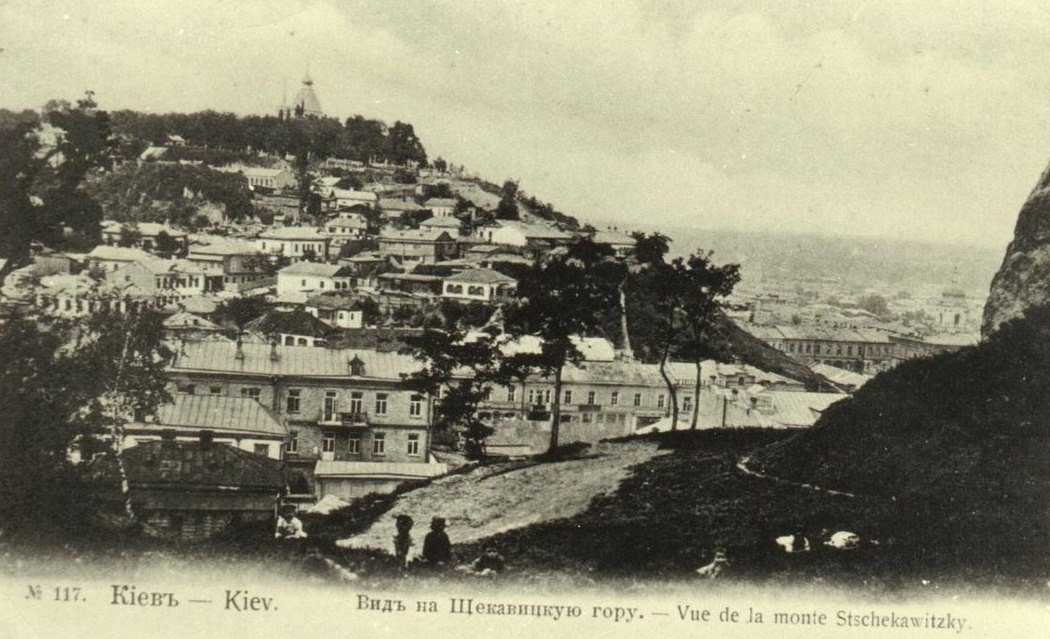
\includegraphics[width=\textwidth]{chast-colebanie-osnov/sheka/sheka-wb.jpg}

%\textit{Вид с нижних уступов Замковой.}
%\end{center}


%А вот скорее всего оконечность улицы Лукьяновской, либо чуть выше, севернее, поворот Олеговской. Прямо по курсу церковь Воздвиженья у подножия Киселёвки:

%\begin{center}
%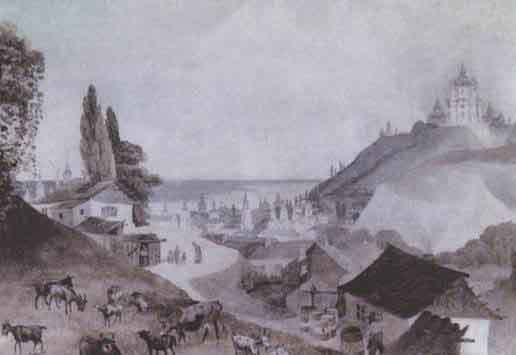
\includegraphics[width=\linewidth]{chast-colebanie-osnov/sheka/sheka-photo.jpg}
%\end{center}


\begin{center}
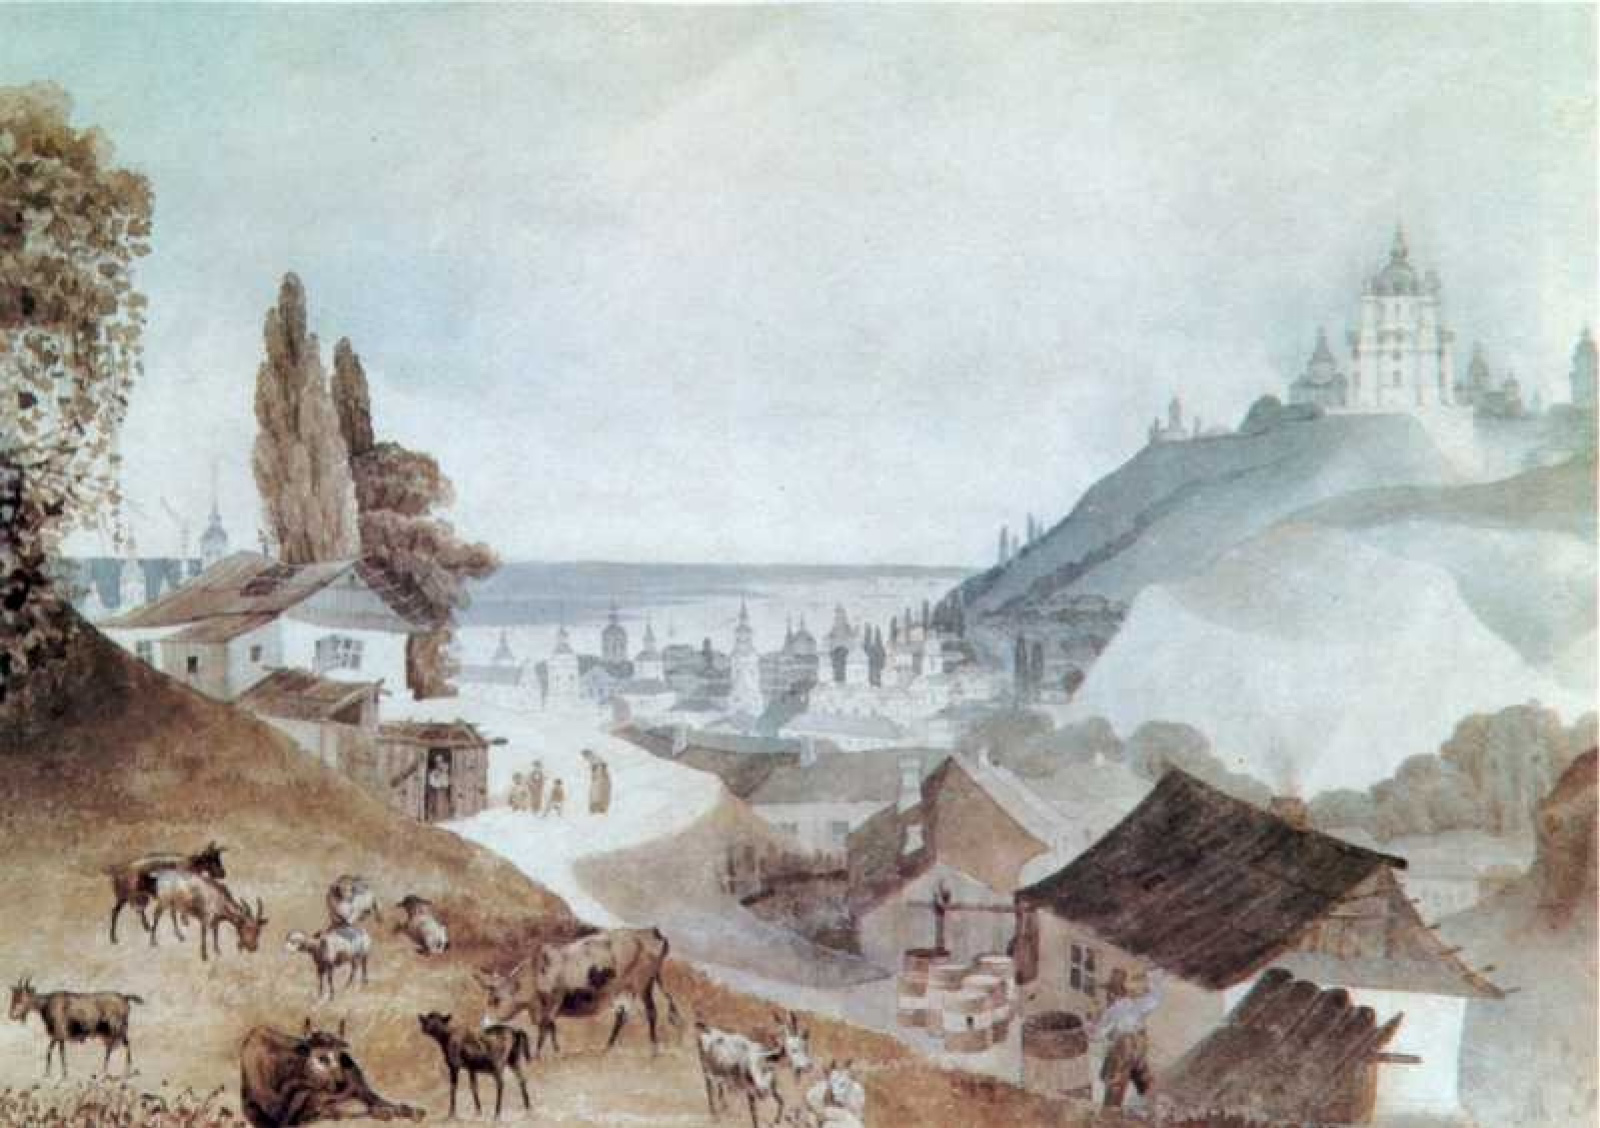
\includegraphics[width=\linewidth]{chast-colebanie-osnov/sheka/sajin-vid-s-shekavici.jpg}

\textit{М. Сажин, "Вид на Подол с Щекавицы", конец 1840-х.}
\end{center}


Кладбище росло, принимая тех, про кого мы не видим память, и тех, чей труд сохранился – например, архитектора Андрея Меленского. Он спроектировал колонну Магдебургскому праву, церковь-ротонду на Аскольдовой могиле, Крестовоздвиженскую церковь возле Киселёвки, Николу Доброго и многое другое. Сам Меленский жил на Подоле, и последний дом его, принадлежащий супруге Меленского, до сих пор стоит на улице Хоревой, под номером 11/13 – это через дорогу от церкви Николы Притиска, около северо-восточного ея угла.

В 1900 году кладбище закрыли, но в советское время на соседнем, уцелевшем старообрядческом кладбище, снова хоронили, и у входа есть братская могила времен Великой Отечественной войны.

Примечательна могила юродивого Ивана Босого (Иван Иванович Расторгуев, 1800-1849)\footnote{Известно еще об одном юродивом Иоанне Босом (Иване Григорьевиче Ковалевском, 1807-1855), погребенном в Китаевой пустыни, а жил он в 1840-х, в Лавре. Тоже босиком ходил, как и многие юродивые. Могила этого Босого не сохранилась.}. Сведения о нем находим у Закревского\cite{zakr01}:

\begin{quotation}
Очевидцы сообщают о нем следующее: Около 1844 г. в двух-этажном доме, составляющем часть фундамента Андреевской церкви, жил некто Иван Босый, уроженец города Зарайска, названный так потому, что ни в какое время года не носил обуви, и в самые лютые морозы его видели босым на улицах Киевских. 

Жизнь свою он посвящал непрестанной молитве и сбору подаяний, употребляя их на содержание в Андреевском доме странников, число которых иногда достигало до двух сот человек. Узнав от бывавших в Киеве поклонниках\footnote{То бишь паломников.}) об этих подвигах благочестия Ивана Босаго, Русь часто слала ему издалека разные приношения и много помогал ему также бывший Киевский губернатор И. И. Фундуклей, оставивший по себе в Киеве память учреждение женской гимназии. 

Этим только может быть объяснено, как мог Босый, без всяких собственных средств, содержать множество поклонников, сменяющихся одни другими. 

Когда он умер, то оказалось, что Босый носил многовесныя железныя вериги, с которыми его и похоронили на горе Щекавице, с большим торжеством. За гробом его шли тысячи народа и слышен был плач многих беспомощных, лишившихся в нем своем подпоры.
\end{quotation}

Был ли Босой старообрядцем, раз могила его на старообрядческом кладбище? Нет, прах перенесли в 1935 году с православного кладбища, когда его уничтожали.

Босой завещал похоронить себя на Щекавице. Его могила еще в 19 веке служила местом паломничества. С нее брали землю, потому она постоянно выглядела взрытой. Максимович и Аскоченский писали в журнальных статьях о встречах с Босым и его поступках.

Лет сорока отроду этот странный человек, прежний мещанин, обыкновенный семьянин стал юродствовать. Скитания привели его в Киев. Одной из особенностей Босого была способность называть незнакомых людей по именам. 

Но о православном кладбище на Щекавице! Руки стали чесаться уничтожить его еще в 1930-х. Хотели разбить парк, как это удалось провернуть с кладбищем у Аскольдовой могилы. Однако, снесли церковь, могилы вокруг, а до парка руки не дошли.

После войны, в 1951 году на кладбище началось строительство вышки-глушилки для подавления радиоэфиров иностранных «голосов». 

%Тоталитарное государство во всесильной злобе своей наделяло трудящихся квартирами, бесплатно их лечило и учило. Отец мой рассказывал – слушал как-то один из «голосов», а там передают, что в Киеве эпидемия и на улицах лежат горы трупов. Выглядывает в окно – да нет, никто не лежит. После этого он ловить «голоса» перестал.

По какой-то безумной причине вышку понадобилось строить именно на Щекавицком кладбище, так же как и сооружать военную часть на соседнем кладбище сверху Замковой горы, телевизионную вместо Еврейского кладбища, участок вьющихся растений в ботсаду на другом Еврейском кладбище, Институт проблем прочности на огромном погребальном холме Братского кладбища, жилой квартал на Воскресенском кладбище, больницу на части Зверинецкого кладбища. Будто полагают, что на костях строить крепче, стоять будет дольше?

Такое варварство – не единоличное решение какого-то заоблачного дяди, а негласный сговор разных «авторов проекта», архитекторов и непосредственных строителей. Все они, получаются, одобряют и поддерживают. Не их родичи там покоятся.

В Питере есть площадь Александра Невского, около Тихвинского кладбища. На северной его околице похоронены композиторы «могучей кучки» – Мусоргский, Балакирев, Бородин, Римский-Корсаков, рядом же могилы Чайковского, Рубинштейна, Даргомыжского, Достоевского. Собственно, на Тихвинском кладбище много кто лежит из великих художников, композиторов, писателей, критиков.

В 1935-37 годах затеяли перепланировку площади и заодно устроили Некрополь мастеров искусств. Так вот площадь расширили, надгробные памятники Мусоргскому, Римскому-Корсакову, Бородину, Балакиреву перетащили в Некрополь, а сами могилы их закатали в асфальт, там сейчас автобусы стоят. Цвет классических композиторов – под асфальт.

После пятидесятых на Щекавице осталось лишь старообрядческое кладбище, на западе горы, в части, выходящей в сторону оврага урочища Юрковицы около районной котельной. Туда мы отправимся позже.

\begin{center}
\includegraphics[width=\linewidth]{chast-colebanie-osnov/sheka/\myimgprefix 27082009558.jpg}

\textit{Снимок 2009 года.}
\end{center}


%В фильме «Киевская сюита» есть сцена, относящаяся к этому кладбищу. Правда, сел аккумулятор камеры и снимать пришлось на мобилу.

В книге Александра Терещенко «Быт русского народа», вышедшей в 1847 году, в главе «Отправление Радунецких поминовений» – в Киеве ныне их называют «гробками» – написано такое:

\begin{quotation}
В Киеве сходились и теперь сходятся на гору Щекавицу не только простой народ, но и почтеннейшие граждане. Там сначала отправляют панихиды над умершими, а потом каждое семейство, сев в кружком близ родственной могилы, поминает родителей, родственников, друзей, знакомых и все, что дорого для их сердца. 

Едят и пьют за упокой, желают усопшим Царствия небесного за их добрые дела; прощают нанесенные им обиды, не желая препятствовать им идти прямо в рай, и просят их не препятствовать им. Когда немножко поразгуляются, тогда заставляют семинаристов или учеников бурсы петь духовного содержания стихи, но печальным и погребальным напевом. Это так трогает настроенную их чувствительность, что они для удержания своих слез запивают горе вином, произнеся: «О, як оце жалостливо! Сховав риднего и ридненьку, хтож мене приголубе? Чи чуете вы, мий батеньку и моя матусенька? Чи вам там лучте, чи нам тутечки?».

После многих возгласов старший из поминальщиков обращается к плачущим и говорит: «Давайте ж скорее чарку горилки – утолым горе!». Когда и это не помогает, тогда обращаются к скрипачам и говорят: «Музыка! Нутеж заиграйте, да так, щоб плакало усе навзрыд». Скрипачи играют заунывные или похоронные песни, и все плачут. «Годи! Чи перестанете ж играты? Не бачете, як вси взрыдалы, мов с изнова риднего хоронют». Скрипачи начинают играть веселые, и все, забыв горе, бросаются вприсядку. 

Поминки обращаются в безотчетный разгул, который иногда продолжается всю ночь. На другой день говорят только: «Ой, болит моя головонька». Чтобы прогнать головную боль, похмеляются; похмелье иногда длится несколько дней сряду. Почти то же самое происходит в Полтавской, Черниговской и Харьковской губерниях.
\end{quotation}

Восточная часть Щекавицы обычно отождествляется краеведами с местностью Бискупщиной. Название это упомянуто лишь в книге Закревского, в земельных документах я его не встречал. Где-то на горе и около, во время владычества Литвы с Польшей были земли, дом и острог бискупа – епископа. В жалованных грамотах можно видеть Бископскую бакшту, Бископский шлях, дом, острог, грунт, но никогда не Бискупщину.

Однако я не договорил об Олеговой могиле. Где же её искать? Сей вопрос беспокоил многих. Максимович в письме Погодину «О горе Щекавице» говорит о своем посещении горы в 1856 году для поиска этой могилы:

\begin{quotation}
И встретился нам, среди несметного множества могил позднейшего времени, презанимательный жилец соседнего удолья. Он привел нас к площадке на северо-восточной стороне горы, и сказал: «Тут была могила Олега!» – сказал с уверенностью, живо напомнившей мне покойного Кондратия Андреевича Лохвицкого\footnote{О деятельности самоуверенного Лохвицкого мы поговорим позже. Впрочем, его самоуверенность в определении древностей ничуть не более таковой у многих современных археологов.}. Что же это указание любопытного киянина: местное предание или недавняя выдумка?
\end{quotation}

Упомянутое Максимовичем место – резко очерченный, явно при участии человека – отрог, почти правильным треугольником вписывающийся между улицами Кирилловской и Нижнеюрковской. 

Туда можно попасть вскарабкавшись на несусветную высоту с задворков Нижнеюрковской, либо, что гораздо проще, идти по Олеговской, миновать вышку, а затем свернуть возле дома номер 36, перед довоенной школой-интернатом, в переулок. Шагать по нему до конца, вдоль малоэтажных старых домов 38, 40 и вперед к гаражам, а по их улочке направо до тупика, там между гаражами будет проход – туда и дальше. 

\begin{center}
\includegraphics[width=\linewidth]{chast-colebanie-osnov/sheka/\myimgprefix IMG_20131117_145800.jpg}

\textit{Ноябрь 2013 года.}
\end{center}

Этот участок горы, если двигаться по Кирилловской к Нижнеюрковской, проглядывает позади зданий, будто обтёсанный великанской лопатой. Фотография сделана с обратной стороны. Местность ископана черными археологами. По склону в траве протоптаны тропки – одни невидимые, но ощутимые ногами, другие столь давние, что глубина их в глинистом грунте доходит до щиколоток. Мы сняли это место на видео в серии «Киевской амплитуды» про Щекавицу.
  
Вершина представляет собой площадку достаточно обширную, чтобы в древности на ней были постройки – град Щека. Установлен некий современный крест, и сооружение из бетонных  цилиндра, призмы, куба, скрепленных треугольником – скульптура 2004 года «Тринити» от «арт-проекта Фиктивная Галерея Экспедиция» Игоря Коновалова. Виднеются ямы – вероятно от давних фундаментов или пещер.

Чуть дальше поворота от Олеговской улицы к этому месту, к Олеговской присоединяется Лукьяновская – и дальше общая дорога продолжается на запад уже как Лукьяновская. У перекрестка до 2020 года был доступ к заасфальтированнму мысу с обрывом, обращенному к горе, подписанной на современных картах как Юрковица. На мысу до 1940 года был татарский базар Шурум-Бурум. Обрыв превращен в свалку. На восток оттуда – современная мечеть, кладбище мусульманское, далее за ним – старообрядческое.

На северных задворках школы в 1988 году нашли пещеру, поныне не исследованную. Среди местных ходила молва про целую сеть пещер в усадьбе этой школы.

На аэрофотоснимке 1943 года я рассмотрел кое-что любопытное. Глядите, отметил малиновой стрелкой.

\begin{center}
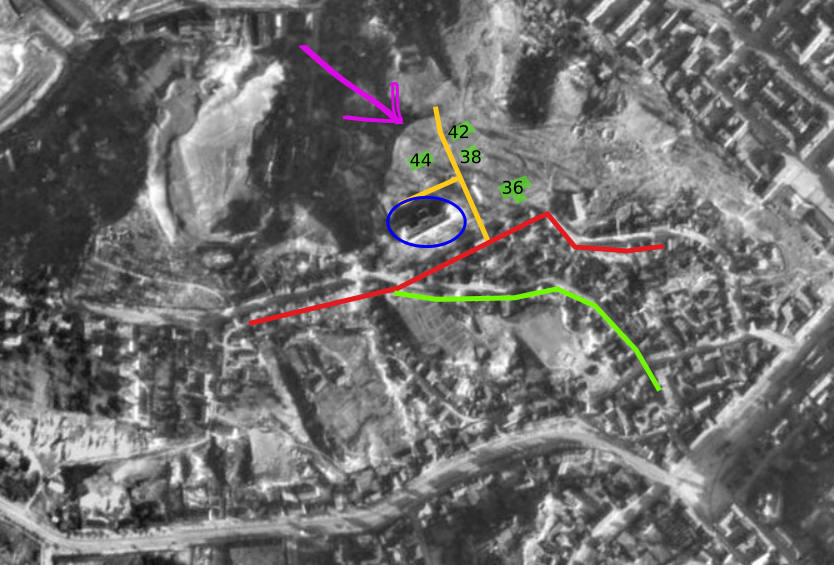
\includegraphics[width=\linewidth]{chast-colebanie-osnov/sheka/she.jpg}
\end{center}

Этот полукруг ныне – в составе усадьбы здания номер 44, а также успешно освоен гаражами. Синим кружком я обвел школу (дом номер 42). Зеленым цветом нарисовал здания, которых не было в 1943. Красная линия – современная Олеговская улица. Как видите, она сдвинута относительно прежней дороги. Желтые линии – заезды мимо школы к домам 44, 42, 38. Зеленая линия – улица Лукьяновская в теперешних пределах, тоже несколько сдвинута.

Согласно плану Щекавицы 1872 года – и школа, и полукруг, и дома были заняты кладбищем. Я не знаю, в произвольном ли порядке изображены на этом плане кресты, или отражают действительное положение каких-то избранных могил. Если первое, то можно сказать – да, пещеры лежали в пределах кладбища, внутри ограды, но мы не знаем, находились ли могилы непосредственно над пещерами. Если второе, то получается, что пещеры покоились под слоем захоронений 19-го и ближайших к нему веков. 

\begin{center}
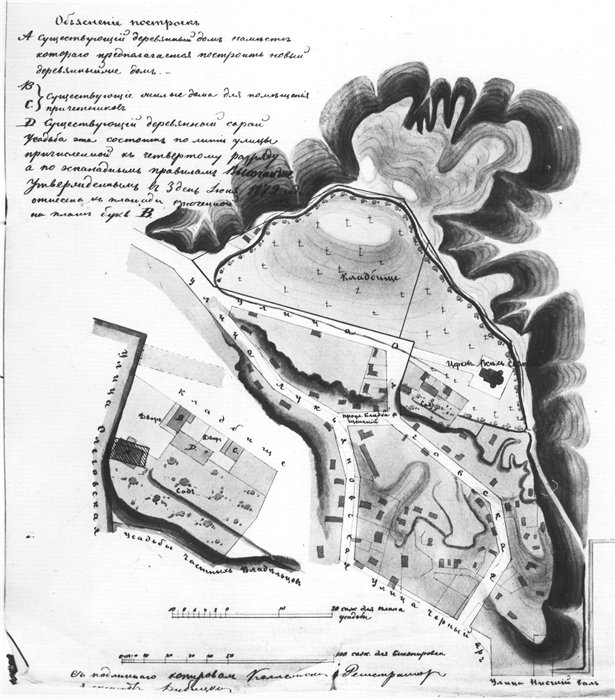
\includegraphics[width=\linewidth]{chast-colebanie-osnov/sheka/1872-shekavica.jpg}
\end{center}

Что же такое полукруг? Внешняя часть некоего пещерного комплекса? Измененные при разбивке кладбища очертания склона? Остаток древнего фортификационного сооружения? Не знаю.

Западнее, на склонах между школой и мечетью, ближе к последней, тоже находились некие пещеры – коридоры с нишами – с погребениями, большей частью уничтоженные при строительстве. Обнаруженные археологом В. К. Гончаровым в начале 1930-х, они так и не были толком изучены, да теперь уж поздно. Вероятно, к этим пещерам примыкали и пещеры в Черном яру – подземный лабиринт с коридорами высотой 1,64 метра, шириной до 0,8, с тремя выходами, да некими кириллическими граффити по стенам. 

А в усадьбе 36-38 на улице Лукьяновской в 1956 году открыли вертикальную шахту полтора на полтора метра, глубиной 14 метров! Куда вела – неясно. Кстати неподалеку, по адресу Лукьяновская 41, археологи нашли, по их словам, фундаменты церкви 12 века, археологический памятник местного значения. Были на Щекавице и другие древние пещеры (одну,  что длилась на глубине 3 метров вдоль юго-восточного склона, удалось проследить на длину 70 метров) – но равнодушие науки и застройка склонов привели к непоправимой их утрате.

Погожим днем 5 июня 2016 года мы с Колей Арестовым отправились на поиски щекавицких пещер. Прежде мы лазали по Щекавице много раз, однако не были вооружены еще знаниями о здешних подземельях. Зеленое лето – не самое лучшее время, чтобы выискивать ямы в земле, однако же выбрались! Тут главное успеть, ведь часть склонов, запечатленных на видео в диком виде еще пару лет назад, уже застроена.

Тихий жилой райончик около школы – особый уголок, его почти не тронуло время. Школа сталинских времен, со стороны Олеговской улицы слишком парадная, с обратной же сохраняет старый дух. Там дворик, граничащий с дорожкой и пустырем, который, отгороженный гаражами, выходит к крупнейшему здешнему зданию – дому номер 44. Всего в околице три домика, о нескольких этажах, прячутся в садовой зелени. Дофига гаражей – гораздо больше, чем жителей! Гаражи выстроились вдоль проулка, обходящего школу с востока, соседствуют со школой к северу, натыканы по упомянутому ранее полукругу, и еще вне его, на возвышении к северу. Возвышение это представляет собой ровный уступ перед следующей к северу террасой.

Во дворе школы никаких входов в пещеры мы не заметили, хотя особо и не искали – уж слишком там всё прилично. На пустыре перед 44-м домом, увидав ямку, мы многозначительно предположили, что в прошлом это возможно был «залаз», но далее этого прозрения истории не продвинулись.

Повстречав местных подростков, мальчика и девочку, я спросил, не знают ли они, где тут пещеры. Мальчик явно знал, но врал, что не знает. Девочка же робко сказала: «может быть там?» – и махнула рукой на запад, но мальчик упорно лукавил, что никаких пещер нет.
 
Исследовать каждый сантиметр местности в пределах видимости мужиков, возящихся с машиной у гаражей, нам не хотелось. Мы стояли в пределах «загадочного полукруга» и ничего не могли поделать. Для изучения нам оставался дикий склон. Мы выбрались к нему привычным ходом между гаражей, в конце эдакой составленной из оных улицы. К этой «улице» от домов на север сходит небольшой спуск. Гаражи\footnote{Гаражи: 50°28'1"N 30°30'9"E} в конце его стоят на террасе, которую я обозначу как Уступ А. Ниже его к северу – другой, превращенный в свалку Уступ Б, предшествующий еще одному, более узкому Уступу – В, за коим идет уже окончательный крутой склон, обращенный к Нижнеюрковской улице.

Таков не весь рельеф этого склона Щекавицы, а лишь его участка непосредственно за упомянутыми гаражами. Весь рельеф слишком сложен, чтобы описать словами, а рисовать у меня нет сил. Добавлю, что описанный ранее северо-восточный отрог Щекавицы с валами и бетонной штуковиной лежит относительно гаражей на северо-восток, а Уступ Б – более на север, соседствуя с упомянутым отрогом.

Пройдя по Уступу Б налево, к западу, под деревьями мы нашли старый раскоп либо обвалившиеся подземные коридоры, в виде буквы «Г»\footnote{\textasciitilde{}50°28'1"N 30°30'8"E}. Глубина его была невелика, в ямах лежал мусор, а уцелевшее рядом сооружение из досок намекало, что именно тут потрудились археологи. Походив между раскопов, мы сняли их на видео для серии «Киевской амплитуды» «Забытые подземелья Киева» и решили продвинуться к Уступу В. 

\begin{center}
\includegraphics[width=0.85\linewidth]{chast-colebanie-osnov/sheka/\myimgprefix IMG_20160605_142252.jpg}
\end{center}

\begin{center}
\includegraphics[width=0.85\linewidth]{chast-colebanie-osnov/sheka/\myimgprefix IMG_20160605_142254.jpg}
\end{center}

\newpage

То бишь со свалки мы двинулись ко склону, в сторону улицы Нижнеюрковской. Поперек пути – крутой спуск, под ним площадка Уступа В, и ниже – еще более крутой, чудесно заросший низенькими вишнями склон. Такие же вишни буйствуют левее. Еще левее и выше – тыл западной части гаражной «улицы».

Там на бугре, в бурьянах, сидели какие-то девочки. Справа же от нас, в некотором удольи, расположилась целующаяся парочка.

Но краеведы имеют право смущать целующихся парочек, если они мешают важной краеведческой работе. Я бы и там, где они лежали, пошарил, но ведь не прогонишь!
 
Мы стали лазать над уступом В, глядеть, что да как, и заприметили ямку.

Для большей ясности. Поросшая травой горка, у ее подножия – уступ, и в нем, под горку уходит некогда большое отверстие, левая половина коего засыпана (но есть щель в подземную пустоту), а правая обвалена, однако не совсем. Это последнее отверстие закидано мусором, подступы же полны битого стекла. Осталась дырка размером наверное с четвертую часть прежнего входа. Пролезть внутрь нельзя, лечь на живот и засунуть туда камеру на длину руки – тоже, из-за стекла и неудобства положения дыры.

Как-то отгребя стёкла, я встал на колени, насколько хватило просунул в отверстие руку и попытался заснять доступные внутренности подземелья сначала на камеру (зажав одновременно в руке фонарик), потом на мобилку (со вспышкой). Последнее получилось несколько удачнее – позже оказалось возможным разглядеть ход налево (вероятно на север). На видео этот коридор не попал, вообще вся съемка велась практически вслепую.

Снимки, которые я помещу далее, стоит разобрать подробно. Других пока не сделал, так что лучшее из худшего. Единственные в мире фотографии древних пещер Щекавицы!

Первый снимок сделан, чтобы вы могли сыскать пещеру самостоятельно. В нижней его части, посередине, есть небольшой куст. Вот за ним-то и скрывается вход. Ближайший в кадре дом, светлая панельная «гостинка» – адрес Нижнеюрковская, 13. Слева от него проглядывает более низкое здание с другой стороны этой улицы, общага, здание номер 4. Это для ориентирования. Ежели будете шляться за гаражами, то когда встретите подобный вид, будете знать, где искать пещеру.

\begin{center}
\includegraphics[width=\linewidth]{chast-colebanie-osnov/sheka/\myimgprefix IMG_20160605_142338.jpg}
\end{center}

\newpage

А этот снимок позволяет оценить высоту склона над уступом В и входом в пещеру. Наверху слева маячит Коля в кепке.
\vspace*{\fill}
\begin{center}
\includegraphics[width=\linewidth]{chast-colebanie-osnov/sheka/\myimgprefix IMG_20160605_142403.jpg}
\end{center}
\vspace*{\fill}
\newpage

\begin{center}
\includegraphics[width=\linewidth]{chast-colebanie-osnov/sheka/\myimgprefix IMG_20160605_142411.jpg}

\textit{Правая часть входа в пещеру.}
\end{center}

   
\begin{center}
\includegraphics[width=\linewidth]{chast-colebanie-osnov/sheka/\myimgprefix IMG_20160605_142437.jpg}

\textit{Внутри.}
\end{center}

\newpage

На последнем снимке я увидел то, что физически не мог рассмотреть, когда фотографировал. Как понятно из предшествующего снимка входа, мне удалось довольно глубоко просунуть руку – ничего, что есть у входа, не попало на внутренний снимок. 

И вот за бутылкой от «Колы», ход идет налево и вероятно понижается, ибо там видна еще одна бутылка либо бутылочка, в кадре много меньшая в сравнении с «Колой». А поскольку таких маленьких бутылочек обычно не бывает, мне кажется, что – «Кола» лежит на светлом краю уступа, а там где темное и бутылочка – это место расположено ниже, и бутылочка просто выглядит маленькой, ибо находится дальше от объектива.

Покамест это всё, что удалось разыскать из пещер на Щекавице. Негусто, а с течением лет и это пропадет, засыпется, обвалится либо будет превращено в свалку. 

Параллельно нынешним Нижнему Валу и Глубочицкой, по холму, устремленные наверх Олеговскую и Лукьяновскую пересекала еще одна улица, Черный яр, названная по урочищу. Она же стыковалась с Лукьяновской еще в одном месте, западнее, подходя к ней внизу посередине между старообрядческим и обычным кладбищами. Следы улицы Черного яра отчетливо сохранялись по 2016 год, на юго-запад от первого поворота Олеговской, за домом Нижний вал, 11. 

На советской карте 1991 года Черный Яр подписан улицей Мирной. Этим названием на дореволюционных и начала 20 века картах обозначена короткая улица от Глубочицкого шоссе наверх к Лукьяновской. Жителям улицы Черный Яр не нравилось именование «Черный Яр». Слишком мрачно. И в 1910 году, по просьбе местных, улица Мирная вобрала в себя б\'ольшую улицу Черный яр и обе улицы стали единой – Мирной – хотя не непрерывной.

Еще в 1980-е, примыкающая к Щекавице сторона улицы Глубочицкой – до перекрестка со Смирнова-Ласточ\-кина (Вознесенский спуск) и дальше по ходу улицы, да параллельная ей Мирная были застроены жилым домами до четырех этажей, но больше по одному-два. Многие здания соединялись впритык. Парадные с деревянными воротами, деревянные же узорчатые обода оконных рам. Почти перед каждым домом – узкий дворик, упирающийся в невысокую опорную стенку, а уже за нею – тротуар улицы. Таким образом первые этажи зачастую были ниже тротуара.

Сейчас там, под крутым склоном Щекавицы – загаженные пустыри. Первыми из строя выбыли дома ближе к Житнему рынку, а точнее к автовокзалу «Подол». На этом месте было прежнее здание базара, приземистое, с полукруглой колоннадой, выходящей к улице Верхний Вал. От прежнего рынка уцелело строение, в котором и поместился автовокзал. Остальное было снесено в 1980 году, причем напротив, под Замковой горой, уже стоял современный новый рынок. А между ними, в небольшом сквере торчали в небо худые тополя. Гремели мимо трамваи.

\begin{center}
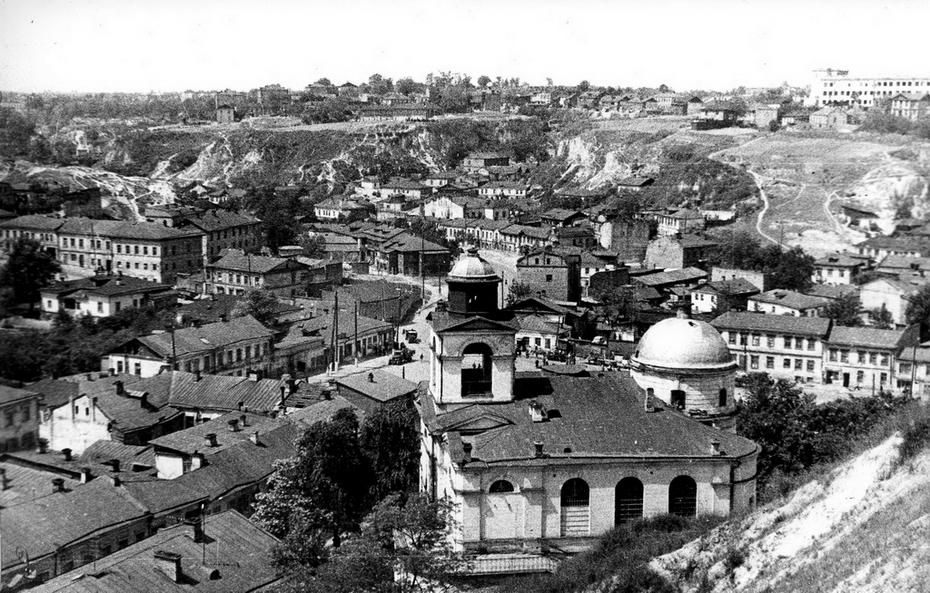
\includegraphics[width=0.95\linewidth]{chast-colebanie-osnov/sheka/0421_KK.jpg}
\end{center}

На снимке 1946 года, сделанном с Киселёвки, прямо за левым куполом Воздвиженской церкви – упомянутое мною начало Глубочицкой, и за нею – Черный яр или Мирная. Здания УТОС слева еще нет. Справа ближе к нам, наискось – склон Замковой, дальше впереди, двумя плоскими подошвами – Щекавица, слева сбегает один из мысков горы Кудрявца.

Если по Лукьяновской, от Нижнего вала подниматься к Олеговской, то по правую сторону есть, срезая угол, лестничка, проход наверх к Олеговской, напротив нынешних домов 32-Б, 32 – существует издавна, по крайней мере с середины 19 века. На 2015 год окрестности охвачены строительством, склоны разрыты. На 2016 – здания уже заслонили этот участок горы.

В девяностых я много ездил к бабушке на Лукьяшу с Подола, восемнадцатым трамваем. Улица Глубочицкая менялась на моих глазах.

Исчезла фабрика игрушек «Победа», имени Карла Маркса, в здании под номером 40. На повороте около завода «Электроприбор», когда улица берет вверх, в вагон проникал мягкий и теплый спиртовый дух – дрожжевого завода. Пару веков назад там был пруд на речке Глубочице, а затем водочный завод Чоколовой. В 2014 году здесь, между Глубочицкой и Татарской улицами, в широком и глубоком яру – огромный пустырь. Поздней осенью 2015-го его стали застраивать жилым кварталом и довершили дело в 2016-м.

Трамвай ездил и ездил, а крутые берега улицы ограждались зелеными заборами. И вырастали за ними не деревья, но здания. И не стало видно склонов, а только бетонные этажи загромождали небо. Прежние строения выбивались, получался пустырь, уходящий вглубь, на склон, от улицы прочь. Сразу обносился он металлическим забором, а в будке селился охранник. Пущать не велено! Частная собственность.

А здорово было кататься поздней осенью, вечером, и глядеть в окно. Возвращаюсь на Подол. Старые здания в желтом фонарном свете. Поднимались сутулые горы. Холодный ветер сорвал с тополей почти все листья. Можно представлять, что бежишь рядом с трамваем, с несусветной скоростью, перепрыгивая преграды. «Улица Солян\'ая!» – объявляет водитель. Сколько разных остановок было, а запомнилось только «улица Соляная!».

%И однажды в начале Олеговской возвёлся чудесным способом дом, который мы с братом окрестили «замком Дракулы». Всё гадали, кто там живет? 

Давно не ездил я по Глубочицкой на трамвае. В последний раз шел по ней пешком, но люди казались лишними. Река машин посередине, припаркованные машины на сером асфальте, многократно отраженный и усиленный берегами автомобильный гул, пыльные тополя.

На западе, у Лукьяновки, уже трудно разделить местности Щекавицы и прилегающих урочих. Это в окрестностях улиц Старая Поляна и проходящая по ложбине яра Соляная. Соляная названа так потому, что раньше тут были солевые колодцы. Их засыпали в первой четверти 20 века. На 2016 год, только северная часть улицы сохранила первозданный вид со старыми домиками. Но всё больше их лежало в развалинах за обочиной, а мимо, по узенькой дороге без тротуара, проносились автомобили.

С запада – спуск по заросшей диким виноградом лестнице от частного сектора на Печенежской, вдоль некоего ручья в коллекторе (в конце 2015 года спуска коснулась уродующая рука разрушения). Около крутого подъема к Лукьяновской – новостройки. Затем Соляная идет в глубоком овраге, в направлении Глубочицкой через гаражный кооператив и промзону (завод «Электроприбор»). На месте промзоны, еще в 1970-х был частный сектор с переулками Соляным, Вишневым и Перекрестным.

Примерно до 1940-х Соляная носила имя Саксоновской, а еще ранее – Саксонский яр и Волчий яр, причем название Саксонского яра улице присвоили еще до революции несмотря на наличие рядом уже существовавшей улицы Саксонский яр. Жители улицы, что ныне слывет Соляной, еще с 19 века называли ее Волчий яр. Почему Волчий яр показан на некоторых картах в районе Нижнеюрковской, там где районная котельная, я не знаю, может там тоже считался Волчий яр, и название переползло на улицу. Что до Саксонского яра, краеведы предполагают, что рядом было кладбище, где хоронили пленённых в ходе войны 1812 года саксонцев. Пленных немецких и французских офицеров в Киеве тогда появилось великое множество. Лечились от ран, ходили на балы, вдоволь ели и пили вместе с такими же идущими на поправку офицерами русскими. Часть пленных затем подалась в учителя и гувернеры.

% Генерал французский Рапп и саксонский Эргард влились в светское общество, рисовали картинки да писали в альбомы стихотворения. Часть пленных затем подалась в учителя и гувернеры.

Но! В 19 веке в Киеве жил и имел немалый общественный вес генерал-фельдмаршал Фабиан Готлиб фон дер Остен-Сакен, чью фамилию часто сокращали до простого Сакена, и порой добавляли в нее лишнее «с» – Саксен. Даже у Михаила Максимовича в автобиографии встречаем такое написание. Может, Саксен владел тут землей, и потому яр назвали Саксонским.

На снимках: улица Соляная в сентябре 2013 года.

\begin{center}
\includegraphics[width=0.90\linewidth]{chast-colebanie-osnov/sheka/\myimgprefix IMG_20130925_164039.jpg}
\end{center}

\begin{center}
\includegraphics[width=0.90\linewidth]{chast-colebanie-osnov/sheka/\myimgprefix IMG_20130925_164327.jpg}
\end{center}
 
\newpage

На плане 1752 года большой овраг между улицей Соляной и Лукьяновской (у номеров 7-А, 9, 11), и далее просто по Соляной, обозначен как «Чертова долина». В эти края мы еще вернемся, когда придет черед поговорить об урочище Юрковице.

%Отрезок Лукьяновской около жилых домов 11, 9, 7 – вдоль знаменитой стены с граффити – это бывшая улица Чмилев яр. Раньше, наверху, где Лукьяновская поворачивает на восток, был перекресток. Старая Поляна с севера соединялась тут с Чмилевым яром (шедшим дальше на юг) и отходящей к востоку Лукьяновской.

%Волчий яр, вопреки мнению, что он на повороте Глубочицкой и между нею и Татарской, да вопреки мнению, что по нему проложена Соляная – находился в другом месте. Так именовали яр под горой непосредственно к северу от Лукьяновской улицы и к западу от Старообрядческого кладбища. Северная сторона Волчьего яра ограничивалась улицей Нижнеюрковской. 

%Волчий яр примыкал к Чмилеву Яру. Волчий яр входит в состав урочища Юрковица. Отрог горы за старообрядческим кладбищем, который считается частью Щекавицы, раньше именовался Юрковицей, позже название это перешло на соседнюю к северу, Лысую гору.

Название Щекавицы принято считать производным от одного из легендарных братьев – Щека.

Некоторые исследователи решили, что слово «щекот» (значащее заливчатое пение птиц, например соловья) – это старинное слово, самого соловья обозначающее. И что-де гора Щековица значит Соловьиная, что там соловьи пели.

Существует еще любопытная история о Щекавице и окрестностях. Я пытался докопаться до источника, однако не смог. Историю эту я знаю по книге М. Возняка «Українські перекази» и отрывочным сведениям из статей.

Сведения гласят, что в 19 веке фольклорист И. Трусевич со слов кобзаря Кирилла записал предание о трех князьях с именами Лукьян, Чикирда и Скавика. Кто такой И. Трусевич? Мне это имя известно лишь по библиографии – в газете «Киевлянин» за 1868 год, из номера в номер печаталась его работа «Предания, поверья, пословицы и песни жителей Полесья». Возняк, вероятно, пересказывает записанную Трусевичем быличку. И вот каким образом:

\begin{quotation}
СКАВИЦЯ
\\
\\
Старі люди кажуть, що тут був гріб князя Скавики. Скавика, Чикирда й Лукіян були начальники, названі князями, лицарського народу, якихось чорноморців, що, як хмари або як сарана, приплили з низу, від моря, до Києва. 

Усі три, разом зі своїми дружинами, поселились на київських горах, один коло одного. Кажуть, що князь Скавика мав дочку, молоду й зовсім непогану дівчину. На його двір збігалися лицарі й королевичі з усіх сторін світу й один перед одним старалися здобути руку княжни. 

Але найкращий, найхоробріший з усіх був князь Чикирда; для княжни вбогий її сусід був миліший від усіх багатств, від усіх корон і берел. Але хоч Скавика сам, як і Чикирда, був князем без князівства, бо стояв тільки на чолі кочовничої орди, все таки бажав собі кращої долі для своєї єдиної дитини та сподівався видати її колись за багатого заморського королевича.

А князь Чикирда посилав сватів, сам навіть падав до ніг Скавики, але це не помогло йому нічого: Скавика жартував собі тільки з бідного молодця. Нарешті вкололо Чикирду таке легковаження і поведінка гордого князька з ним, отже добув свій булатний меч і на ньому присяг помсту своєму ворогові. А князь Лукіян тим часом виглядав лиш відповідної і догідної хвилини, бо й він давно вже мріяв про те, щоб знищити сусідніх князьків і щоб самому заволодіти Києвом. 

Отже як тільки ворожі дружини напали на себе, Лукіян мінами висадив частину військ обої князів у повітря, а решту знищив мечами. Скавика й Чикирда відгадали намір Лукіяна й, подавши собі руки, з'єднаними силами напали на свого спільного ворога. Але більша частина їх військ згинула вже від мін. Отже по довгій й кривавій боротьбі з'єднані дружини враз із своїми провідниками зостались на полі бою.

А найгірший з трьох був Лукіян; він не щадив навіть жінок і дрібних дітей, саму гарну дочку Скавики вбив своєю власною рукою. Тіла провідників похоронили на двох сусідніх горах, а Лукіян лишивсь єдиним володарем Києва.

Глибокі печери на Лукіянівці покопали Лукі\-янові дружини. Кажуть, що пізніше, в часі нападу татарів, вони служили за сховок для бідних киян, бо невірна татарва гнала молодших і сильніших в ясир, а решту забивала на місці. Їх орди ставали звичайно обозом за містом, бо в місті не було місця для них: огонь пожирав усе до грунту. 

Місцевість, в якій татари розбивали свої намети, служила їм тільки для складування здобичі і для варення харчів, тому й назвали її Приваркою.
\end{quotation}

Сделаю некоторые примечания. Местность Приварка – искаженное Приорка. Лежит на западе Оболонского района. Поселение в ней основал (настоятель) доминиканского конвента святого Николая, Петр Розвадовский. 

Лукьяновка именуется, как приняли с подачи Закревского, от Лукьяна Александровича, цехмейстера подольских сапожников, здешнего жителя и землевладельца конца 17 века.

Прежде Лукьяновкой считали, в общем, всю горную местность к западу от Кирилловских высот и около, например Репяхов яр. Отдельные части Лукьяновки слыли под разными именами вроде Верхней Юрковицы. На Лукьяновке выделилась местность Татарка (частично совпавшая с Верхней Юрковицей), занимающая район между улицами Печенежская, Половецкая, Отто Шмидта и Подгорной. Основной же магистралью ее проходит улица Татарская.

Овраг с улицей Нижнеюрковской на плане 1752 года овраг подписан «Унизовая долина». Современная улица, на отрезке примерно от ее соединения с Отто Шмидта, и далее вниз с горы, до 1837 года носила имя Чикирдин спуск. Чикирда – довольно распространенная фамилия, и спуск мог именоваться по землевладельцу, а вот значение слова неясно. Возможно чекирда – это искаженное «шакирд» (учащийся медресе, мусульманского учебного заведения). Не зря же местность – Татарка.
%Некоторые полагают, что оно образовано от среднеазиатского «чигиря» или «чикира», колесного устройства для подъема воды на высоту, чтобы поливать сады-огороды. А возможно чекирда – это искаженное «шакирд» (учащийся медресе, мусульманского учебного заведения). Не зря же местность – Татарка. Чикирдин спуск – Шакирдин спуск. Предположение.

Что в приведенной истории про Скавику от Возняка, а что от кобзаря или Трусевича, я не ведаю. И потом, не надо воспринимать кобзарей как хранителей преданий, точнейшим образом передающих из поколения в поколение исторические события. Творчество кобзарей было нескольких видов – народным, затем, из «учено-культурной» среды («господа» сочиняли думы и обучали им кобзарей) и, наконец, поддельным. Слишком мало данных, чтобы сделать вывод.

\newpage
\vspace*{\fill}
\begin{center}
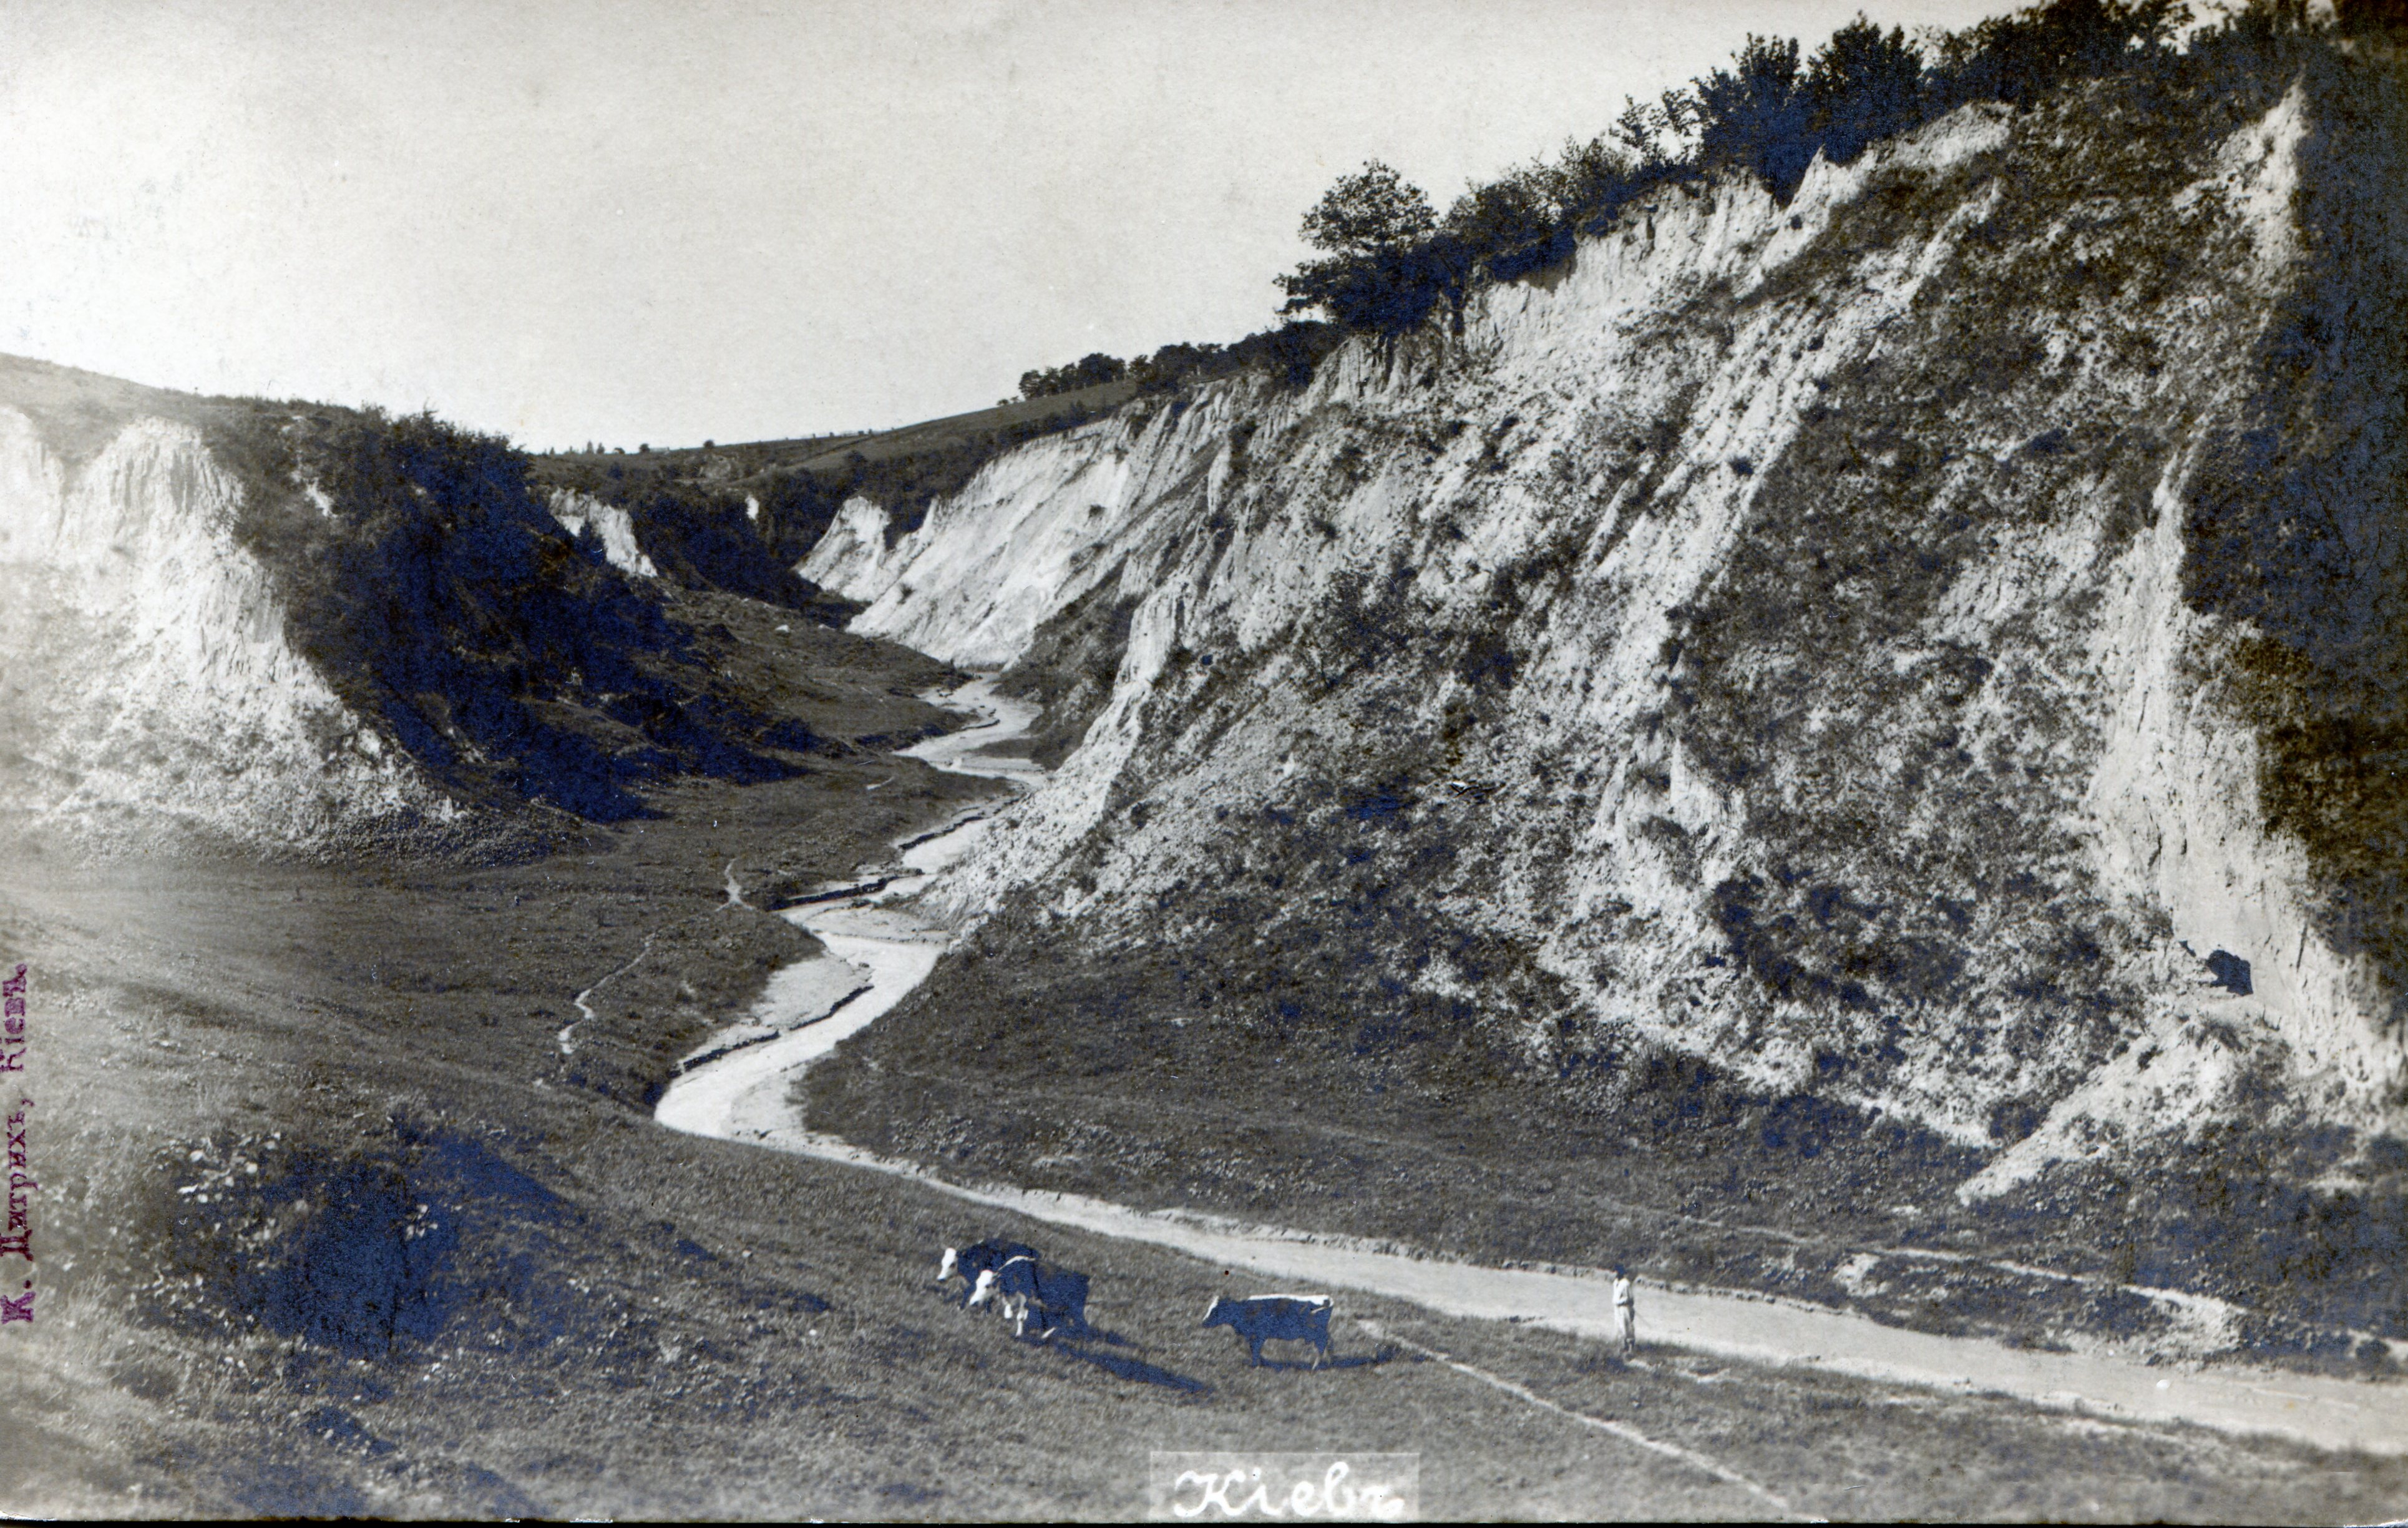
\includegraphics[width=\linewidth]{chast-colebanie-osnov/sheka/lukold01.jpg}
\end{center}

\begin{center}
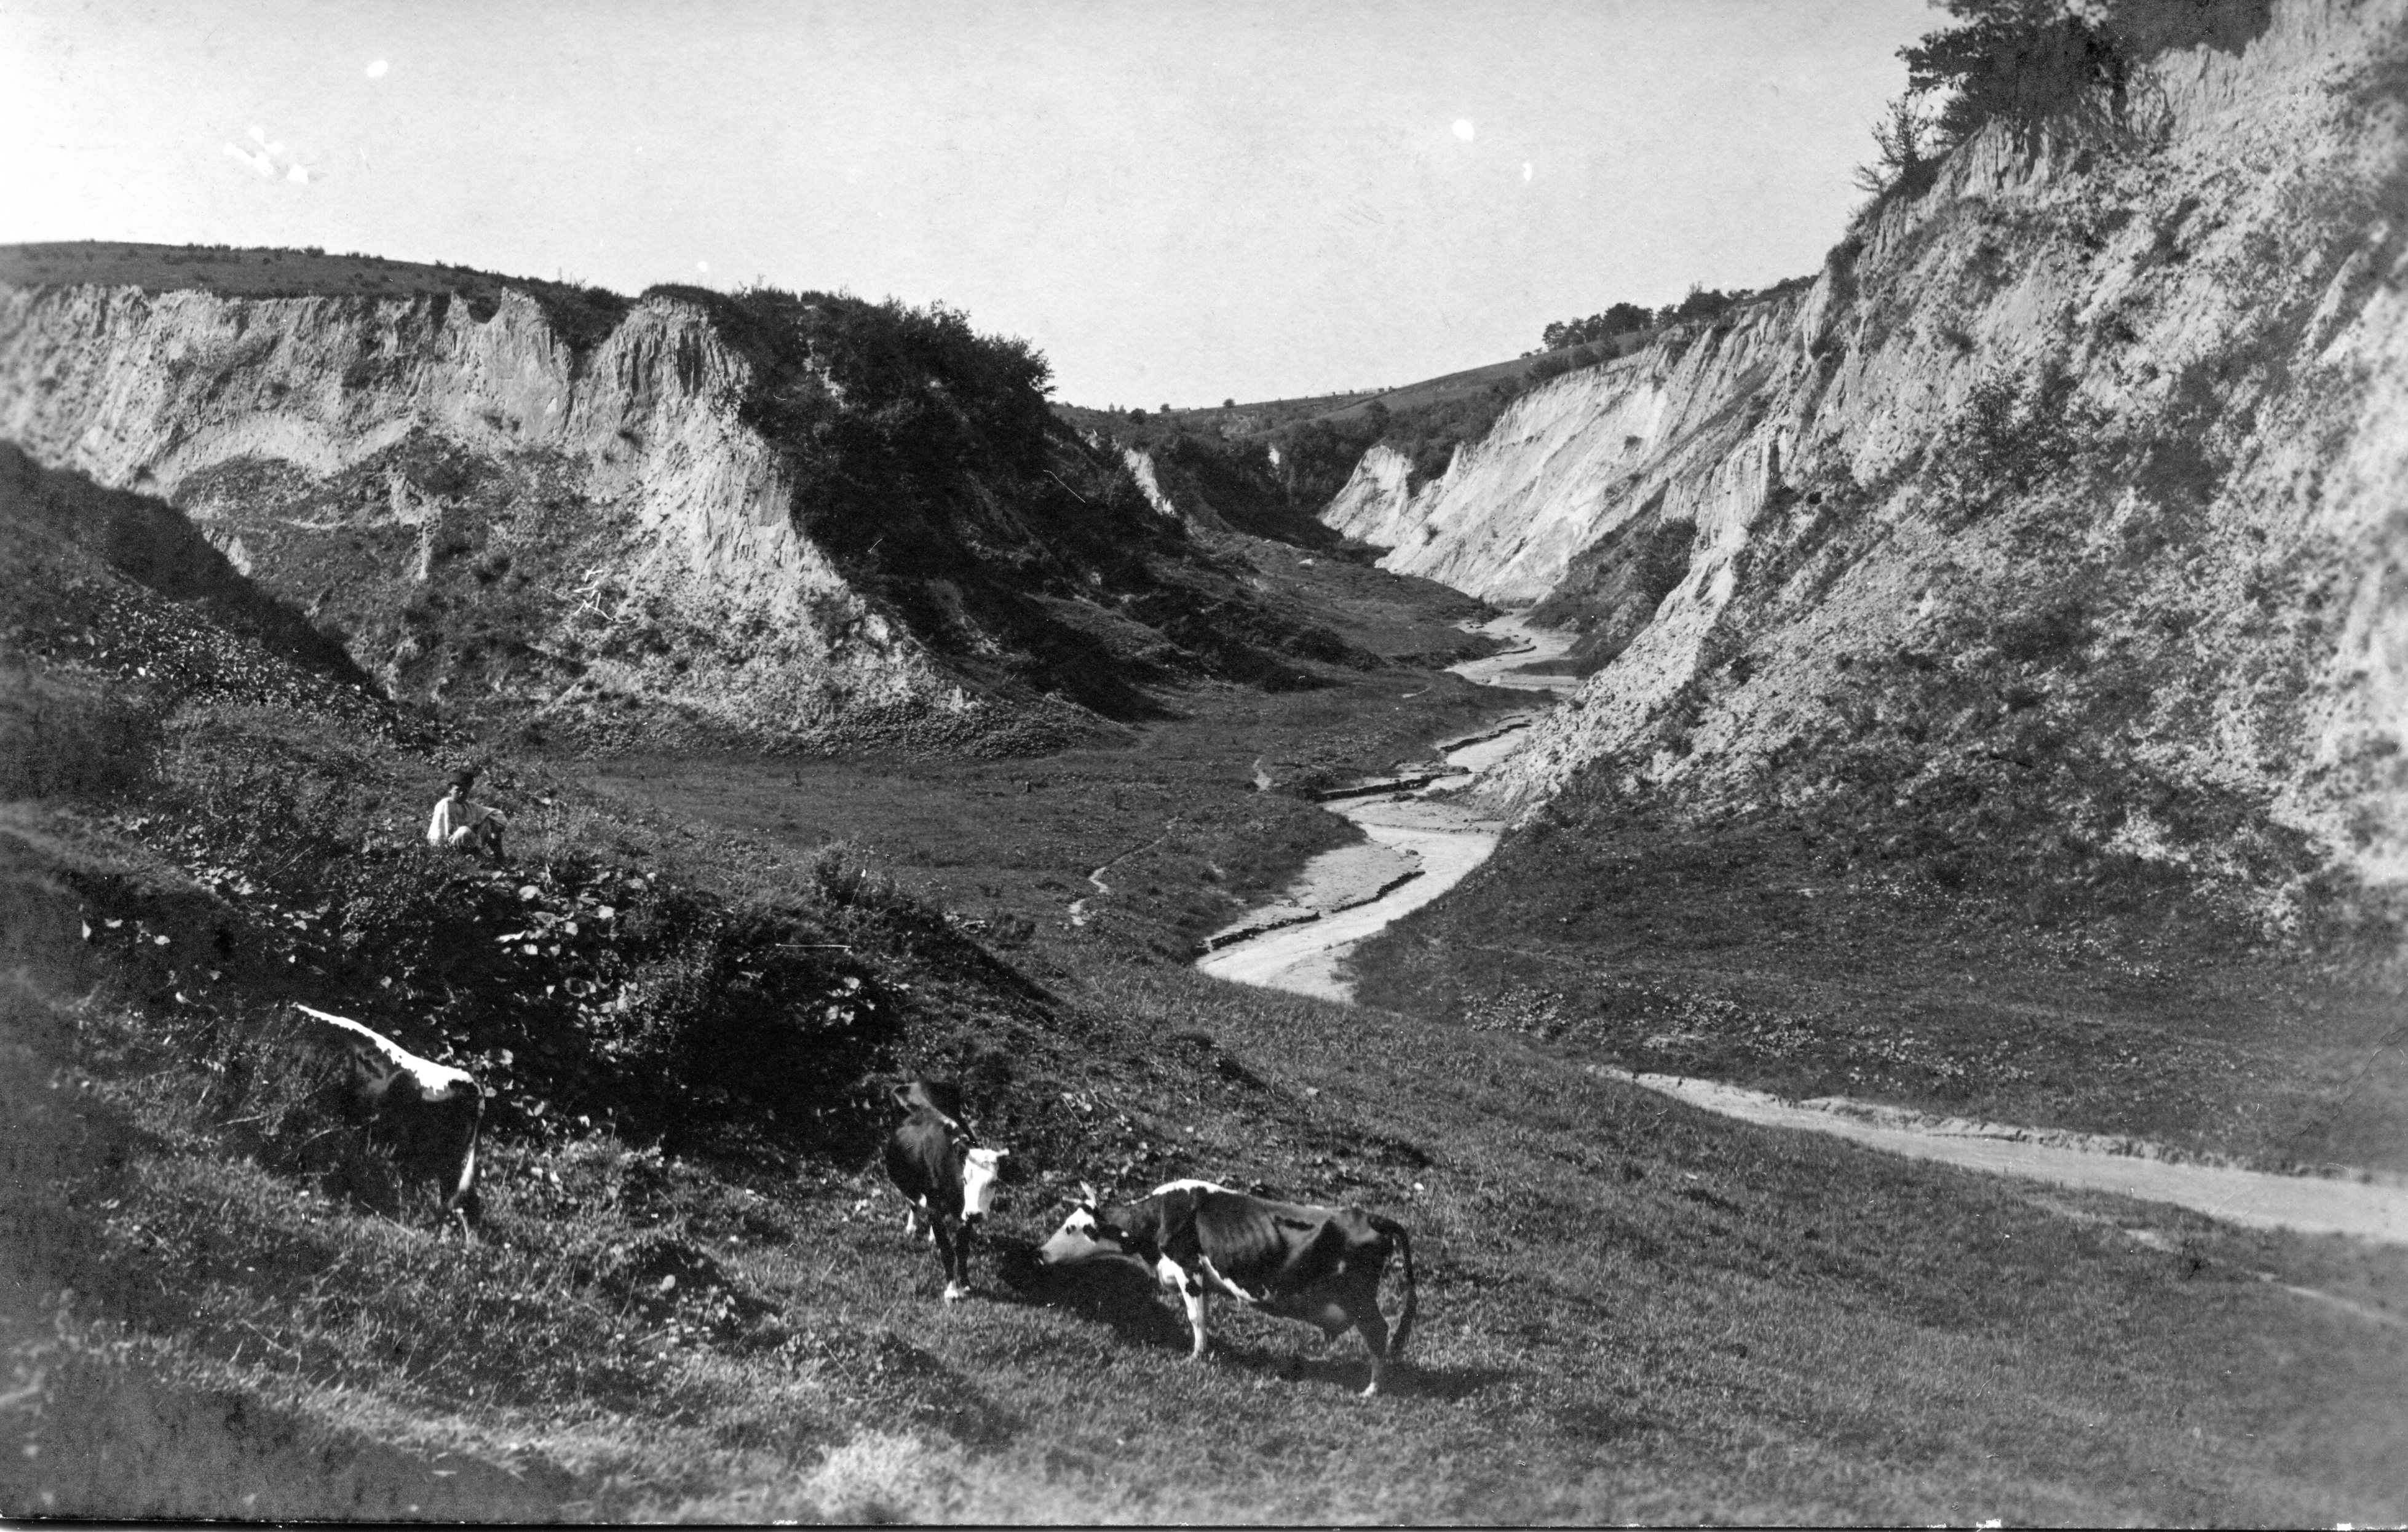
\includegraphics[width=\linewidth]{chast-colebanie-osnov/sheka/lukold02.jpg}

\textit{19 век, в снимках предполагается «Лукьяновка». Возможно, Репяхов или Бабий яр.}
\end{center}
\vspace*{\fill}
\newpage

В именах Скавика и Лукиян угадываются искаженные Щек и Кий (довольно отбросить «лу» и получим Киян). Любопытно упоминание о князьях как о «черноморцах», слова про пещеры на Лукьяновке.

Судьба застроенной Щекавицы могла сложиться совершенно иначе. Гора бы теперь была музеем.

В 1861 году умер Тарас Шевченко и сначала его погребли в Питере. Но почитатели решили уважить стихотворное желание поэта быть похороненным на Украине. Спустя два месяца гроб вырыли, взломали, увидали, что плесенью покрылся Тарас. В другой, свинцовый ящик заточили. Повезли.

Хотели похоронить в Киеве. Занимался хлопотами троюродный брат Тараса, Варфоломей. Хоронить собирались именно на Щекавице, но потом, опасаясь студенческих демонстраций при этом, решили устроить более келейное погребение при Выдубицком монастыре, переправив тело на лодке с левого берега, когда свинцовый гроб подвезут к Цепному мосту. 

6 мая, в последний миг всё переиначили. Варфоломей объявил, что петербуржское общество настаивает, дабы по воле покойника могила была на горе между Каневом и Пекарями, на берегу Днепра. Надобно отметить, что в тех краях Тарас долго и безуспешно пытался взять в долговременную аренду землю, чтобы построить себе хату и наконец осесть. Воли же Шевченко, который вовсе не собирался умирать, быть там похороненным не было.

Гроб с телом Шевченко после панихиды в Рождественской церкви (на Почтовой площади) по набережной перенесли к пароходу «Кременчуг», стоящему подле Цепного моста. Так попрощался Тарас Шевченко с Киевом, в последний раз проплывая мимо мест, которые некогда рисовал.

И в Канев! Вопреки той же стихотворной воле «Як умру, то поховайте мене на могилі серед степу широкого», похоронили Шевченко не в степи, а на горе Чернечьей под Каневом, и не на древнем кургане, а насыпав новый курган над гробом. 

Кстати при жизни, с 1840-х, Шевченко часто бывал на Подоле, его хорошо помнили торговки-«сидухи» около Братства, грубо говоря, бурсы. И вот эти сидухи уже после смерти поэта рассказывали чудесное, будто ездит Шевченко по Подолу на белом коне. 

Посмертно он, своей могилой, защитил бы Щекавицу от разорения.
